\chapter{Implementation and Performance Evaluation of Neural Networks For Index Acceleration}
\label{ch:implementation-evaluation}

In the previous chapter, we have presented the neural network based algorithm to accelerate the partial tuple search of relational data.  Our algorithm relies on a partial tuple classifier to optimize the ordering of text index search.  In particular, we have shown that a variety of neural network architectures can be used in the design of the classifier.

In this chapter, we will describe the evaluation of the proposed solutions.  We will verify the effectiveness and limitations of our solutions, and perform a comparative study of different network architectures.  For each network architecture, we will present the benefits and drawbacks, and provide our understanding of the explanation of the observations.

\section{Some assumptions about datasets}
\label{sec:assumption}
In this section, we list some assumptions for our experimental evaluation:
\begin{itemize}
	\item The numbers of tuples of relations are not skewed, this is, there is no relation that has an extremely large number of tuples than other relations.
	\item Applying operations of inserting new tuples, updating or deleting existing tuples to a database does not introduce new vocabulary.
\end{itemize}

These assumptions imply limitations of our proposed solutions. We will provide some discussion about the limitations and possible future work in Section~\ref{sec:limitation}.

\section{Datasets}
The datasets we have used to evaluate our system is a collection of survey data from Statistics Canada \cite{ds01, ds02, ds03, ds04, ds05, ds06, ds07, ds08, ds09, ds10}, which includes one labour force survey, six COVID-19 surveys, one income survey, one community health survey, and one housing survey.
They offer many real-world characteristics that pose as challenges to  neural network classifiers.  Given the intended application scenarios of our research, we felt that it was important to evaluate our work using real-world datasets. For easy reference in subsequent sections, we give each dataset an id, as shown in Table \ref{table:id_name}.   
\begin{table}[t]
	\centering
	\begin{tabularx}{\textwidth}{|l|X|}
		\hline
		\textbf{Dataset id} & \textbf{Dataset name} \\
		\hline
		ds01 & Labour Force Survey, April 2019 [Canada] \\
		ds02 & Crowdsourcing: Impacts of COVID-19 on Canadians’ Experiences of Discrimination Public Use Microdata File \\
		ds03 & Crowdsourcing: Impacts of COVID-19 on Canadians Public Use Microdata File, [2020] \\
		ds04 & Crowdsourcing: Impacts of the COVID-19 on Canadians – Your Mental Health Public Use Microdata File, [2020] \\
		ds05 & Crowdsourcing: Impacts of COVID-19 on Canadians' Perception of Safety Public Use Microdata File, [2020] \\
		ds06 & Crowdsourcing: Impacts of the COVID-19 on Canadians – Trust in Others Public Use Microdata File [2020] \\
		ds07 & Impacts of the COVID-19 pandemic on postsecondary students (ICPPS) 2020, Crowdsource file, Public use microdata file \\
		ds08 & Canadian Income Survey (CIS), 2017 \\
		ds09 & Canadian Community Health Survey - Annual Component (CCHS) 2017-2018 \\
		ds10 & Canadian Housing Survey, 2018 \\
		\hline
	\end{tabularx}
	\caption{Dataset ids and names}
	\label{table:id_name}
\end{table}

These 10 datasets contain both numerical and textual data with different numbers of attributes and tuples. For example, the labour force survey contains data of the Canadian labour market. It has total 60 attributes related to the job market, such as employment status, industry, status of working full-time or part-time, hourly wage, etc. Table \ref{tab:ds01_samples} shows 5 samples with a subset of 10 attributes. The descriptions of the selected 10 attributes are shown in table \ref{tab:ds01_attrs_samples}.
\begin{table}[!ht]
	\centering
	\resizebox{\textwidth}{!}{%
		\begin{tabular}{
				|c
				|c
				|>{\raggedright\arraybackslash}p{0.1\textwidth}
				|>{\raggedright\arraybackslash}p{0.1\textwidth}
				|l
				|>{\raggedright\arraybackslash}p{0.2\textwidth}
				|>{\raggedright\arraybackslash}p{0.2\textwidth}
				|>{\raggedright\arraybackslash}p{0.2\textwidth}
				|l
				|l|}    \hline
			\multicolumn{1}{|c|}{\textbf{survyear}} &
			\multicolumn{1}{c|}{\textbf{survmnth}} &
			\multicolumn{1}{c|}{\textbf{lfsstat}} &
			\multicolumn{1}{c|}{\textbf{prov}} &
			\multicolumn{1}{c|}{\textbf{age\_12}} &
			\multicolumn{1}{c|}{\textbf{educ}} &
			\multicolumn{1}{c|}{\textbf{immig}} &
			\multicolumn{1}{c|}{\textbf{noc\_10}} &
			\multicolumn{1}{c|}{\textbf{ftptmain}} &
			\multicolumn{1}{c|}{\textbf{hrlyearn}} \\ \hline
			2019 &
			April &
			Employed, at work &
			Ontario &
			25 to 29 years &
			Postsecondary certificate or diploma &
			Non-immigrant &
			Natural resources, agriculture and related production occupations &
			Full-time &
			33.00 \\
			2019 &
			April &
			Not in labour force &
			British Columbia &
			70 and over &
			Bachelor\Verb|''|s degree &
			Non-immigrant &
			&
			&
			\\
			2019 &
			April &
			Employed, at work &
			British Columbia &
			45 to 49 years &
			High school graduate &
			Non-immigrant &
			Business, finance and administration occupations &
			Full-time &
			26.00 \\
			2019 &
			April &
			Employed, at work &
			Ontario &
			20 to 24 years &
			Postsecondary certificate or diploma &
			Non-immigrant &
			Health occupations &
			Full-time &
			37.60 \\
			2019 &
			April &
			Employed, at work &
			Ontario &
			70 and over &
			Some postsecondary &
			Immigrant, landed more than 10 years earlier &
			Occupations in art, culture, recreation and sport &
			Part-time &
			32.00 \\ \hline
		\end{tabular}%
	}
	\caption{5 samples from the labour force survey dataset ``ds01", showing only 10 attributes.}
	\label{tab:ds01_samples}
\end{table}
\begin{table}[t]
	\centering
	\begin{tabular}{|l|l|}
		\hline
		\multicolumn{1}{|c|}{\textbf{Attribute}} & \multicolumn{1}{c|}{\textbf{Description}}     \\ \hline
		survyear & Survey year                        \\
		survmnth & Survey month                       \\
		lfsstat  & Labour force status                \\
		prov     & Province                           \\
		age\_12  & Five-year age group of respondent  \\
		educ     & Highest educational attainment     \\
		immig    & Immigration status                 \\
		noc\_10  & 2016 NOC (10 categories)           \\
		ftptmain                                 & Full- or part-time status at main or only job \\
		hrlyearn & Usual hourly wages, employees only \\ \hline
	\end{tabular}
	\caption{10 attributes and their descriptions from the labour force survey dataset ``ds01".}
	\label{tab:ds01_attrs_samples}
\end{table}
Table \ref{table:ds_stats} shows the number of attributes and tuples in each dataset.
\begin{table}[t]
	\centering
	\begin{tabular}{ |l|r|r|r|r|r|r|r|r|r|r| }
		\hline
		\textbf{Dataset id} & \textbf{No. of attrs.} & \textbf{No. of tuples} \\
		\hline
		ds01 & 60 & 100,885 \\
		ds02 & 129 & 36,662 \\
		ds03 & 47 & 242,512 \\
		ds04 & 43 & 45,989 \\
		ds05 & 23 & 43,631 \\
		ds06 & 47 & 36,538 \\
		ds07 & 42 & 101,902 \\
		ds08 & 194 & 92,286 \\
		ds09 & 1051 & 113,286 \\
		ds10 & 132 & 61,750 \\
		\hline
	\end{tabular}
	\caption{Number of attributes and tuples in each dataset.}
	\label{table:ds_stats}
\end{table}

Sometimes different datasets share common attributes. For example, the COVID-19 datasets have a common attribute about community size and metropolitan influence zones where the survey correspondents live in. By using multiple partial tuple completion, users can ``jump" from one dataset to another. For example, users may find some data related to discrimination from the dataset of impacts of COVID-19 on Canadians’ experiences of discrimination. Then they can use the results to search more information about people's perception of safety in the communities with the same sizes in the dataset of impacts of COVID-19 on Canadians’ perception of safety. This will help users to gain more insights from the survey results.

\section{Architecture and software stack}
In order to thoroughly evaluate the end-to-end search system, we have developed a platform with the following technology stack.  We use Lucene \cite{lucene} as the full-text index.  A customized search engine is developed on top of Lucene to support partial tuple search queries.  This is necessary for us to have detailed instrumentation to collect performance metrics, and to gain control over the ordering of text index search.  We have implemented all neural network based classifiers using TensorFlow \cite{tensorflow}. The trained models are used to generate the ordering of Lucene index access. 
The evaluation of the neural network acceleration is based on the speed-up of query performance between the machine learning generated ordering and other alternatives.
In addition, top-$k$ accuracy is also used to evaluate models.
The query workloads used in evaluation are generated from the datasets themselves. Figure \ref{fig:proj_arch} shows the high-level architectural overview of our implementation. More details about the training datasets and the query workload generation will be presented in subsequent sections.
\begin{figure}[!th]
	\centering
%	\includesvg[inkscapelatex=false, width = 250pt]{overall_architecture.svg}
	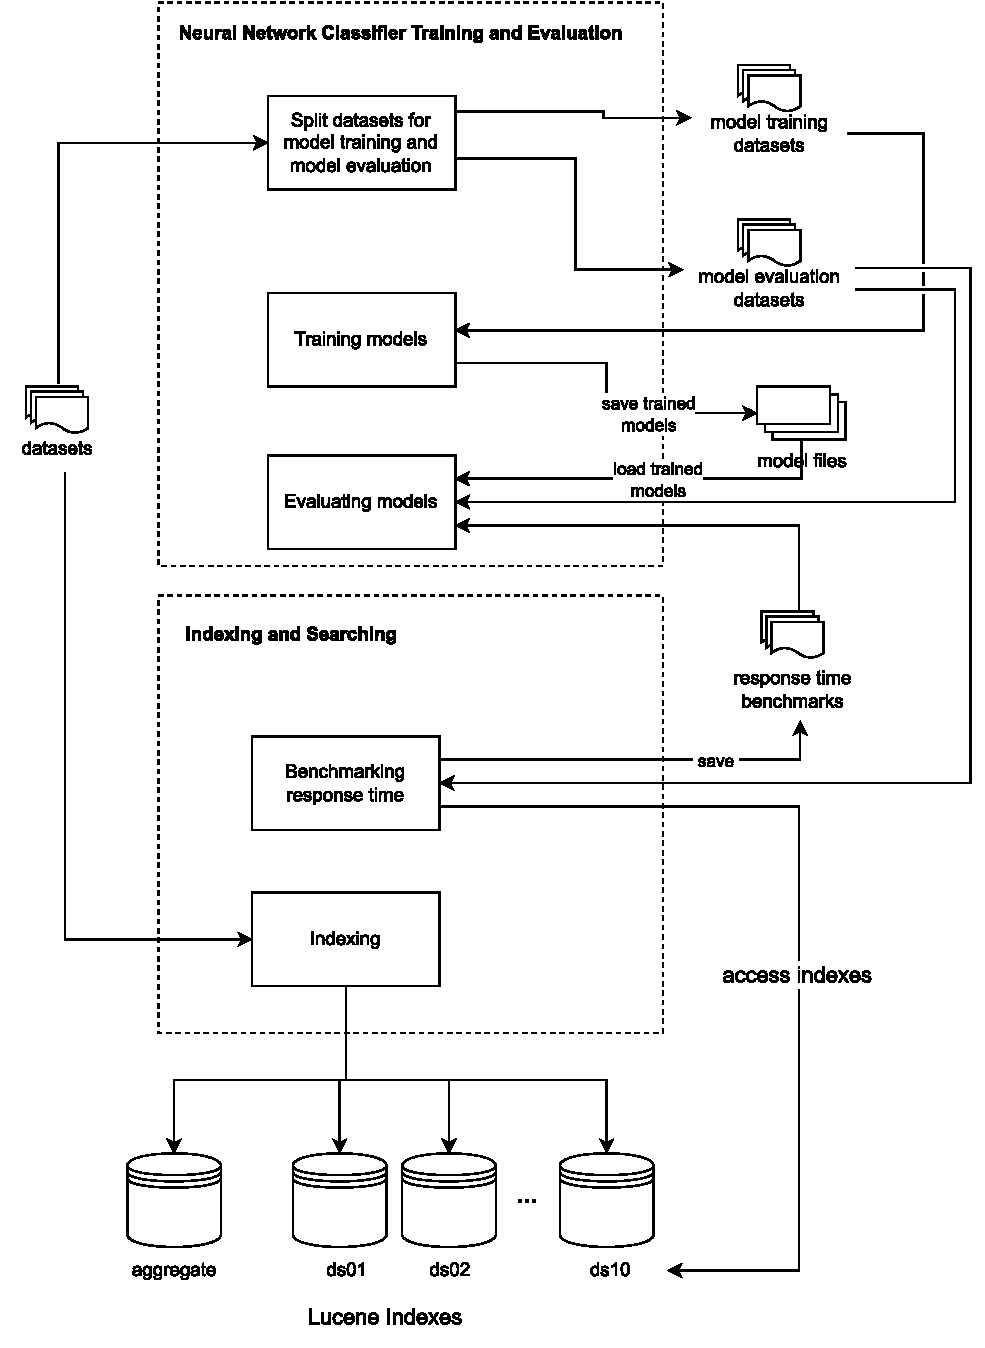
\includegraphics[width=0.8\textwidth]{my/graphics/overall_architecture.pdf}
	\caption{High-level overview of architecture}
	\label{fig:proj_arch}
\end{figure}

\subsection{Lucene and a customized search engine}
We developed a customized search engine on top of Lucene. It has two main functions. The first is to index datasets to create Lucene indexes. 
When indexing datasets, each tuple is converted to a Lucene document, which contains a set of \emph{(attribute name, attribute value)} pairs. We apply character-based 3-gram tokenization to attribute values. We use the special character ``\_" for padding. In addition, we add an extra field ``fulltext" to the document, which contains all 3-gram tokens of all attribute values. This field is needed to support full-text search.
For example, given a tuple $t$ as, 
$$
\{\mathrm{Name}:Jack,\ \mathrm{Gender}:Male,\ \mathrm{Occupation}:\makebox{Software developer}\}
$$
our search engine will first apply Lucene's standard tokenization, and then our character-based 3-gram tokenization. The resulting Lucene document will be,
$$
\left[\begin{array}{rl}
\mathrm{name}: & \_\_j\ \_ja\ jac\ ack\ ck\_\ k\_\_ \\
\mathrm{gender}: & \_\_m\ \_ma\ mal\ ale\ le\_\ e\_\_ \\
\mathrm{occupation}: & \_\_s\ \_so\ sof\ oft\ ftw\ twa\ war\ are\ re\_\ e\_\_\ \_\_d\ \_de\ dev\ eve\ vel \\
& elo\ lop\ ope\ per\ er\_\ r\_\_ \\
\mathrm{fulltext}: & \_\_j\ \_ja\ jac\ ack\ ck\_\ k\_\_\ \_\_m\ \_ma\ mal\ ale\ le\_\ e\_\_\ \_\_s\ \_so\ sof \\
& oft\ ftw\ twa\ war\ are\ re\_\ e\_\_\ \_\_d\ \_de\ dev\ eve\ vel\ elo\ lop\ ope \\
& per\ er\_\ r\_\_
\end{array}\right]
$$

The second main function is to support partial tuple search queries. We also use character-based 3-gram tokenization when constructing a search query. For example, given a partial tuple as:
$$
\{\mathrm{Name}:Jack,\ \mathrm{Gender}:Male\}
$$
the search query will be:
$$
\{\mathrm{fulltext}: \_\_j\ \_ja\ jac\ ack\ ck\_\ k\_\_\ \_\_m\ \_ma\ mal\ ale\ le\_\ e\_\_\}
$$

\subsection{Partitioned indexes and an aggregate index}

We have indexed the tuples from all datasets into a single Lucene index.  The tuples are tokenized  using the 3-gram tokenizer in order to support fuzzy string matching as described in Section~\ref{sec:fuzzy-collision}.  This index will be referred to as the {\em aggregate index} since it contains all the tuples from 10 datasets in a single index.  The aggregate index contains approximately 877,000 documents.

We also have an alternative way of indexing the tuples using Lucene.  We partition the tuples based on which relation they belong to.  Given that we have 10 datasets, we have created 10 individual indexes, each containing the tuples from their respective relation.  We refer to the set of indexes as {\em partitioned indexes}.
The number of documents in each partitioned index is the same as the number of tuples in each dataset, as shown in Table \ref{table:ds_stats}.

With the two types of indexing schemes (partitioned vs aggregate indexing), we have many alternatives in evaluating a user query.

\noindent {\bf Aggregate index lookup:} we can simply issue the user query against the aggregate index as it contains all the available tuples.  

\begin{itemize}
    \item Pro: This is the traditional approach. It requires the least system design. Only a single thread is needed for each user query.
    \item Con: As we have indicated previously and will show in our experimental evaluation, this approach suffers from a performance bottleneck resulting from high token hashing collision rate.
\end{itemize}

\noindent {\bf Parallel lookup of partitioned indexes:} we can issue the query against all individual index in the partitioned index set.  This will perform parallel index lookup using multiple concurrent threads.

\begin{itemize}
    \item Pro: The result can be found quickly.  The index with the {\em correct} tuple will contain much less documents compared to the aggregate index, and thus will respond with the search result faster.  In fact, we argue that this is the optimal performance one can expect.
    \item Con: The concurrency will impose a higher CPU and disk IO demand as each user query will take up to $n$ threads to process.  In high traffic or low resource scenarios, this may be prohibitively expensive.
\end{itemize}

{\noindent \bf Predictive sequential lookup of partitioned indexes}: we advocate to perform single threaded  access of the partitioned indexes.  But rather than simple or random sequential scan of the index set, we utilize predictive neural networks to generate an optimized access pattern, as described in Section~\ref{sec:opt_pipeline}.

\begin{itemize}
    \item Pro: This method enjoys the advantage of both single-threaded index lookup and  low disk latency due to the potential early hit in a smaller partitioned index.  So we argue that the predictive lookup will yield high query performance and low resource usage.
    \item Con: This method requires a self-supervised neural network to perform the prediction.
\end{itemize}

\section{Evaluation methodology}
We evaluate five model architectures, including Multilayer Perceptron (MLP), Long Short-Term Memory (LSTM), 1D Convolution (Conv1D), Transformer and MLP-Mixer. We also exam how misspelled keywords affect the models' top-5 accuracies.

We use two metrics for model evaluation. The first metric is query processing time. We submit queries to partitioned indexes and the aggregate index, and record the response times as evaluation benchmark. More details are given in the subsection \ref{subsection:perf_baseline_expt}.

The second metric is top-$k$ accuracy. A model's prediction gives us the ordering of Lucene index access. If the Lucene index that a query belongs to is among the top-$k$ of the model's prediction, we consider the prediction accurate. For example, for a query sampled from \verb|ds02|, if the predicted access ordering is 
\begin{verbatim}
idx_ds06, idx_ds10, idx_ds07, idx_ds05, idx_ds02, ...
\end{verbatim}
we consider it an accurate top-5 prediction.

In the following subsections, we give more details about our training data, query workloads and experiments. We first describe how training data and query workloads are generated and tokenized in subsections \ref{subsection:training_data_gen} and \ref{subsection:query_workload_gen}, respectively. 
After that, we describe our experiments in subsections starting from  \ref{subsection:perf_baseline_expt} to  \ref{subsection:expt_3gram_resiliency}.

\subsection{Training data generation and tokenization}
\label{subsection:training_data_gen}
The raw datasets are in SAS7BDAT format, which is a binary database format. To make data processing easier for the downstream model training and evaluation, we convert all raw datasets to CSV files. Then we remove some unuseful attributes. For example, the labour force survey dataset contains the attribute \emph{rec\_num}, which indicates the record number in the file. This attribute is removed since it is not useful for our model training. After that the preprocessed CSV files are splitted into data for model training and data for model evaluation. Data for model evaluation are used to generate query workloads. More details about the query workloads generation will be presented in subsection \ref{subsection:query_workload_gen}.

Our next step is to generate training datasets from data reserved for model training. We randomly sample tuples from each CSV file without replacement. Then we normalize the sampled tuples to lowercase and remove special characters from them, which gives us word-based training data. In addition, we also apply character-based 3-gram tokenization to normalized tuples. We use ``\_" as the special character for padding in our implementation.  This results in 3-gram based training data. For example, given a raw tuple:
\begin{verbatim}
(2019,April,"Employed, at work",Nova Scotia,Other CMA or non-CMA,
45 to 49 years,,Female,Married,Above bachelor''s degree,
"Single jobholder")
\end{verbatim}
the normalized tuple will be:
\begin{verbatim}
(2019,april,employed at work,nova scotia,other cma or non cma,
45 to 49 years,female,married,above bachelors degree,
single jobholder)
\end{verbatim}
and the 3-gram tokenized tuple will be:
\begin{verbatim}
(__2 _20 201 019 19_ 9__,__a _ap apr pri ril il_ l__,__e _em emp mpl
plo loy oye yed ed_ d__ __a _at at_ t__ __w _wo wor ork rk_ k__,__n 
_no nov ova va_ a__ __s _sc sco cot oti tia ia_ a__,__o _ot oth the 
her er_ r__ __c _cm cma ma_ a__ __o _or or_ r__ __n _no non on_ n__ 
__c _cm cma ma_ a__,__4 _45 45_ 5__ __t _to to_ o__ __4 _49 49_ 9__ 
__y _ye yea ear ars rs_ s__,__f _fe fem ema mal ale le_ e__, __m _ma
mar arr rri rie ied ed_ d__,__a _ab abo bov ove ve_ e__ __b _ba bac
ach che hel elo lor ors rs_ s__ __d _de deg egr gre ree ee_ e__,__s
_si sin ing ngl gle le_ e__ __j _jo job obh bho hol old lde der er_
r__)
\end{verbatim}
Since we evaluate our models using partial tuple queries, a natural question is whether training models using partial tuples will have any impact on models' performance. Therefore, besides training datasets containing full tuples, we also create datasets containing partial tuples with 75\% and 50\% of attributes. Since each dataset will have an additional 3-gram tokenzed version, we have total six sets of training datasets. Table \ref{tab:training_vocab_size} shows their vocabulary sizes. In addition, we use dataset names as labels, so there is no need to manually label training tuples.
\begin{table}[t]
	\centering
	\resizebox{\textwidth}{!}{%
		\begin{tabular}{|l|ll|ll|ll|}
			\hline
			\multirow{2}{*}{\textbf{}} &
			\multicolumn{2}{c|}{\textbf{100\% attrs.}} &
			\multicolumn{2}{c|}{\textbf{75\% attrs.}} &
			\multicolumn{2}{c|}{\textbf{50\% attrs.}} \\ \cline{2-7} 
			&
			\multicolumn{1}{l|}{word-based} &
			3-gram based &
			\multicolumn{1}{l|}{word-based} &
			3-gram based &
			\multicolumn{1}{l|}{word-based} &
			3-gram based \\ \hline
			\multicolumn{1}{|c|}{vocabulary size} &
			\multicolumn{1}{r|}{56,482} &
			\multicolumn{1}{r|}{4,136} &
			\multicolumn{1}{r|}{47,536} &
			\multicolumn{1}{r|}{4,130} &
			\multicolumn{1}{r|}{37,183} &
			\multicolumn{1}{r|}{4,109} \\ \hline
		\end{tabular}%
	}
	\caption{Vocabulary size of six sets of training datasets.}
	\label{tab:training_vocab_size}
\end{table}

\subsection{Query workload generation and tokenization}
\label{subsection:query_workload_gen}
Query workloads are sets of partial tuples. 
We first randomly sample tuples from data reserved for model evaluation. 
Then we apply the same normalization process to them as we do to training datasets. 
After that we convert them to partial tuples by randomly sampling some attributes from them.
We create different workloads by varying the number of attributes sampled.
Table \ref{tab:workloads} shows two query workloads we used for model evaluation.
\begin{table}[t]
	\centering
	\begin{tabularx}{0.8\textwidth}{|l|X|}
		\hline
		\textbf{Workload name} & \textbf{Description} \\ \hline
		workload A & 5 randomly sampled attributes \\
		workload B & 3 randomly sampled attributes \\
		\hline
	\end{tabularx}
	\caption{Query workload names and descriptions.}
	\label{tab:workloads}
\end{table}

\subsubsection{Converting partial tuples to Lucene queries for searching}
We use Lucene's Query API to construct search queries from partial tuples. First we apply 3-gram tokenization to a partial tuple to get a list of tokens. Then we convert each token to a search term. After that we use the logical \verb|OR| operator to combine all search terms to form a query.
For example, given a partial tuple as the following:
\begin{verbatim}
no very easy no
\end{verbatim}
by adding the character ``\_" for padding, the constructed query will be:
\begin{verbatim}
__n OR _no OR no_ OR o__ OR __v OR _ve OR ver OR ery OR ry_ OR y__ OR
__e OR _ea OR eas OR asy OR sy_ OR y__ OR __n OR _no OR no_ OR o__
\end{verbatim}

\section{Experiments and observations}

In this section, we will enumerate over the experiments we conducted to evaluate our methodology.  For each experiment, we will focus on the motivation, experimental setup, the observation and their respective conclusions.

\subsection{Performance of aggregate vs optimal index lookup}
\label{subsection:perf_baseline_expt}
\noindent{\bf Description:}

Our first experiment tries to establish a baseline for the evaluation of our methodology using the query processing time. We measure three types of performance. The first is the optimal performance, which is achievable by parallel partitioned indexes lookup. The second is the performance of the aggregate index lookup. The last is the performance of sequential scan of all partitioned indexes. This will be the worst sequential scan if the predicted ordering of index access from our neural network classifiers puts the true partitioned index, i.e., the one contains the tuple, as the last one to scan.

To create the performance benchmark, we perform search against partitioned indexes and the aggregate index using the constructed partial tuple queries and log the response times. We repeat the process 10 times and compute the mean response times to be used as benchmark for model evaluation. Table \ref{tab:benchmark_A} and \ref{tab:benchmark_B} show the mean response times in milliseconds (ms) of the first 20 queries of the workload A and B, respectively. Both of the workloads have 1,000 queries. In both tables, the first 10 columns are the results of partitioned indexes, and the last one is that of the aggregate index. Details about the query workloads are described in subsection \ref{subsection:query_workload_gen}.
\begin{table}[!th]
	\centering
	\resizebox{\textwidth}{!}{%
		\begin{tabular}{|c|r|r|r|r|r|r|r|r|r|r|r|}
			\hline
			\textbf{} &
			\multicolumn{1}{c|}{\textbf{idx\_ds01}} &
			\multicolumn{1}{c|}{\textbf{idx\_ds02}} &
			\multicolumn{1}{c|}{\textbf{idx\_ds03}} &
			\multicolumn{1}{c|}{\textbf{idx\_ds04}} &
			\multicolumn{1}{c|}{\textbf{idx\_ds05}} &
			\multicolumn{1}{c|}{\textbf{idx\_ds06}} &
			\multicolumn{1}{c|}{\textbf{idx\_ds07}} &
			\multicolumn{1}{c|}{\textbf{idx\_ds08}} &
			\multicolumn{1}{c|}{\textbf{idx\_ds09}} &
			\multicolumn{1}{c|}{\textbf{idx\_ds10}} &
			\multicolumn{1}{c|}{\textbf{idx\_agg}} \\ \hline
			0  & 46.57   & 18.074  & 11.766 & 12.315 & 11.681 & 10.991 & 8.146   & 32.037 & 42.178  & 12.506 & 171.814 \\
			1  & 9.785   & 95.191  & 9.112  & 3.577  & 5.211  & 5.076  & 42.509  & 25.545 & 11.406  & 8.152  & 34.883  \\
			2  & 41.464  & 30.662  & 15.134 & 7.381  & 9.833  & 6.114  & 16.265  & 25.711 & 130.263 & 28.414 & 340.52  \\
			3  & 81.665  & 71.147  & 10.45  & 11.374 & 13.238 & 62.585 & 24.985  & 33.262 & 89.623  & 22.483 & 214.195 \\
			4  & 11.86   & 12.193  & 4.124  & 3.576  & 2.569  & 4.466  & 5.933   & 14.683 & 10.914  & 7.414  & 27.807  \\
			5  & 111.691 & 35.233  & 23.712 & 14.259 & 37.553 & 32.163 & 90.013  & 38.077 & 64.649  & 56.575 & 410.775 \\
			6  & 10.171  & 15.061  & 6.72   & 6.757  & 5.178  & 6.366  & 20.423  & 9.027  & 17.965  & 13.738 & 48.165  \\
			7  & 8.565   & 17.936  & 3.222  & 11.276 & 3.91   & 9.101  & 12.828  & 8.33   & 29.897  & 50.721 & 113.489 \\
			8  & 4.702   & 2.492   & 3.492  & 2.109  & 1.748  & 2.76   & 1.972   & 10.48  & 6.715   & 5.909  & 18.459  \\
			9  & 29.805  & 25.247  & 4.121  & 3.972  & 3.618  & 8.858  & 21.882  & 65.882 & 40.683  & 97.196 & 403.81  \\
			10 & 12.438  & 28.071  & 11.567 & 7.722  & 8.266  & 8.296  & 17.631  & 25.093 & 28.216  & 30.15  & 69.155  \\
			11 & 78.894  & 199.486 & 36.34  & 16.409 & 59.3   & 19.544 & 52.956  & 31.944 & 81.945  & 49.079 & 269.655 \\
			12 & 34.995  & 17.869  & 6.531  & 8.366  & 4.515  & 9.189  & 11.174  & 38.777 & 33.707  & 16.754 & 98.553  \\
			13 & 27.613  & 291.843 & 36.575 & 18.002 & 16.23  & 21.494 & 10.564  & 35.939 & 35.287  & 9.281  & 513.177 \\
			14 & 14.984  & 19.801  & 18.374 & 7.259  & 9.394  & 10.142 & 11.601  & 10.555 & 24.247  & 5.859  & 181.814 \\
			15 & 13.587  & 7.268   & 3.283  & 4.145  & 2.499  & 3.895  & 11.989  & 9.273  & 72.258  & 10.647 & 210.635 \\
			16 & 13.702  & 95.056  & 9.045  & 3.973  & 5.103  & 8.488  & 38.507  & 36.359 & 12.235  & 17.131 & 49.995  \\
			17 & 56.258  & 33.413  & 15.297 & 20.917 & 77.721 & 36.136 & 20.222  & 23.676 & 60.217  & 25.79  & 200.614 \\
			18 & 82.657  & 47.663  & 13.094 & 16.612 & 20.459 & 22.733 & 250.602 & 23.769 & 66.409  & 15.952 & 349.091 \\
			19 & 54.616  & 101.808 & 19.846 & 10.232 & 17.782 & 10.651 & 15.67   & 20.257 & 31.221  & 18.2   & 170.922 \\ \hline
		\end{tabular}%
	}
	\caption{Mean query processing time in milliseconds of the query workload A.}
	\label{tab:benchmark_A}
\end{table}
\begin{table}[!th]
	\centering
	\resizebox{\textwidth}{!}{%
		\begin{tabular}{|c|r|r|r|r|r|r|r|r|r|r|r|}
			\hline
			\textbf{} &
			\multicolumn{1}{c|}{\textbf{idx\_ds01}} &
			\multicolumn{1}{c|}{\textbf{idx\_ds02}} &
			\multicolumn{1}{c|}{\textbf{idx\_ds03}} &
			\multicolumn{1}{c|}{\textbf{idx\_ds04}} &
			\multicolumn{1}{c|}{\textbf{idx\_ds05}} &
			\multicolumn{1}{c|}{\textbf{idx\_ds06}} &
			\multicolumn{1}{c|}{\textbf{idx\_ds07}} &
			\multicolumn{1}{c|}{\textbf{idx\_ds08}} &
			\multicolumn{1}{c|}{\textbf{idx\_ds09}} &
			\multicolumn{1}{c|}{\textbf{idx\_ds10}} &
			\multicolumn{1}{c|}{\textbf{idx\_agg}} \\ \hline
			0  & 98.113 & 57.467  & 10.403 & 37.902 & 12.051 & 62.483 & 38.51   & 26.149 & 165.856 & 16.691  & 314.936 \\
			1  & 14.557 & 55.388  & 28.667 & 5.697  & 9.935  & 7.249  & 11.154  & 12.134 & 71.949  & 8.198   & 238.055 \\
			2  & 8.631  & 3.937   & 3.175  & 2.545  & 5.582  & 2.101  & 9.151   & 4.998  & 15.669  & 4.413   & 67.788  \\
			3  & 11.335 & 102.476 & 9.366  & 3.973  & 5.219  & 5.831  & 43.672  & 31.271 & 11.799  & 10.532  & 38.502  \\
			4  & 5.308  & 3.488   & 1.841  & 1.794  & 1.599  & 1.831  & 2.318   & 5.721  & 5.43    & 4.208   & 16.736  \\
			5  & 3.67   & 3.528   & 1.455  & 0.888  & 1.378  & 1.309  & 1.754   & 3.788  & 5.68    & 5.098   & 7.443   \\
			6  & 91.594 & 71.66   & 13.706 & 19.588 & 13.286 & 26.387 & 19.932  & 34.864 & 100.266 & 149.223 & 534.203 \\
			7  & 31.022 & 8.103   & 3.399  & 3.869  & 10.046 & 19.07  & 24.614  & 21.792 & 12.224  & 21.41   & 79.365  \\
			8  & 12.886 & 2.355   & 1.921  & 1.164  & 1.289  & 1.857  & 2.255   & 21.522 & 13.225  & 8.419   & 57.589  \\
			9  & 22.284 & 24.1    & 5.037  & 5.806  & 5.746  & 6.755  & 29.814  & 47.61  & 18.798  & 95.213  & 123.481 \\
			10 & 15.28  & 100.405 & 18.486 & 22.014 & 10.342 & 14.922 & 23.115  & 46.89  & 71.578  & 44.932  & 257.194 \\
			11 & 25.516 & 112.658 & 16.634 & 7.536  & 10.233 & 3.534  & 10.162  & 23.997 & 23.325  & 17.062  & 208.747 \\
			12 & 10.205 & 14.475  & 2.911  & 8.536  & 14.028 & 10.525 & 28.727  & 13.78  & 13.006  & 6.637   & 144.816 \\
			13 & 22.995 & 37.862  & 31.601 & 5.188  & 6.149  & 12.015 & 13.627  & 12.671 & 37.18   & 7.093   & 263.558 \\
			14 & 19.333 & 17.295  & 22.824 & 9.389  & 7.053  & 8.066  & 14.066  & 14.804 & 28.168  & 12.026  & 143.885 \\
			15 & 19.342 & 15.851  & 17.527 & 8.61   & 10.577 & 10.279 & 6.839   & 13.137 & 94.481  & 5.259   & 151.432 \\
			16 & 14.672 & 6.689   & 3.557  & 3.29   & 5.204  & 5.284  & 8.676   & 4.322  & 17.68   & 4.766   & 98.075  \\
			17 & 37.963 & 110.194 & 27.724 & 24.375 & 57.606 & 39.03  & 10.182  & 58.863 & 56.036  & 16.456  & 235.116 \\
			18 & 53.005 & 31.016  & 6.474  & 14.265 & 10.915 & 30.343 & 160.273 & 9.875  & 18.179  & 11.012  & 263.5   \\
			19 & 8.122  & 40.389  & 4.695  & 2.191  & 19.547 & 7.517  & 8.134   & 6.303  & 25.256  & 9.781   & 56.903  \\ \hline
		\end{tabular}%
	}
	\caption{Mean query processing time in milliseconds of the query workload B.}
	\label{tab:benchmark_B}
\end{table}

\noindent{\bf Observations:} 

As shown in figures \ref{fig:agg_vs_partitioned_A} and \ref{fig:agg_vs_partitioned_B}, the mean values of processing times of the worst sequential scan are longer than that of searching the aggregate index. The worst sequential scan is slower than searching the aggregate index by 45\% and 35\%, respectively. The goal of our neural network classifiers is to improve the performance of sequential scan by generating an optimized access pattern.
\begin{figure}[!th]
	\centering
	\begin{subfigure}{0.45\textwidth}
		\centering
		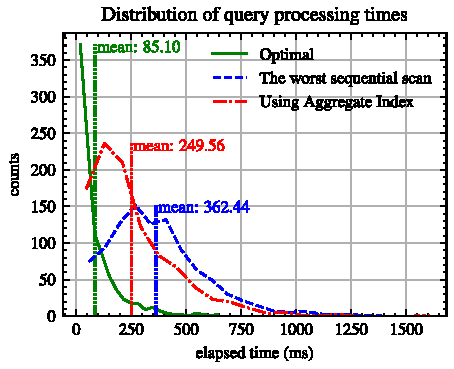
\includegraphics[]{my/graphics/agg_vs_partitioned_A.pdf}
		\caption{Workload A}
		\label{fig:agg_vs_partitioned_A}
	\end{subfigure}
	\hfill
	\begin{subfigure}{0.45\textwidth}
		\centering
		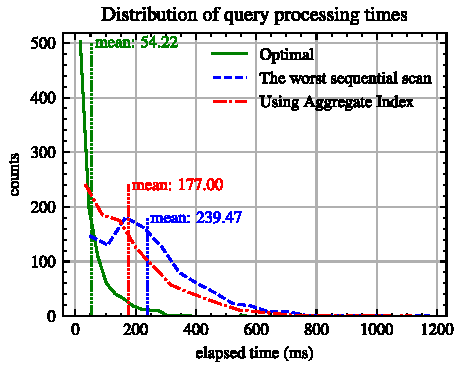
\includegraphics[]{my/graphics/agg_vs_partitioned_B.pdf}
		\caption{Workload B}
		\label{fig:agg_vs_partitioned_B}
	\end{subfigure}
	\caption{The distribution of query processing times of workload A and B.}
	\label{fig:agg_vs_partitioned_all}
\end{figure}

\subsection{Performance of optimal matching for partial tuple completion}
In this experiment, we examine the performance of optimal matching in three different steps.
In our first step, we set query size to be 10, tuple size to be 200, and edge connectivity density to be 0.1. We compute the optimal matching for 100 times and record the response times. Figure~\ref{fig:tuple_completion_1} shows the histogram of the results.
\begin{figure}[!th]
	\centering
	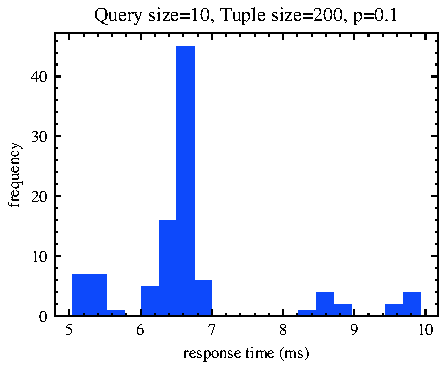
\includegraphics[width=0.6\textwidth]{my/graphics/tuple_completion_1.pdf}
	\caption{Distribution of optimal matching response times (ms)}
	\label{fig:tuple_completion_1}
\end{figure}
In our second step, we vary edge connectivity densities with the same fixed query size and tuple size as in step one. We repeat the process 100 times and compute the mean response times as results, which are shown in Figure~\ref{fig:tuple_completion_2}.
\begin{figure}[!th]
	\centering
	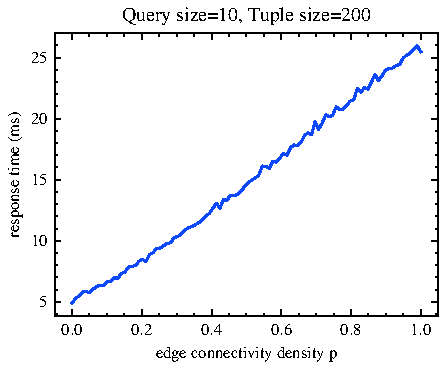
\includegraphics[width=0.6\textwidth]{my/graphics/tuple_completion_2.pdf}
	\caption{Optimal matching response time (ms) w.r.t. varying edge connectivity densities}
	\label{fig:tuple_completion_2}
\end{figure}
In our last step, we fix the query size and edge connectivity density to be the same as in step one, but change the tuple size so that it goes from 100 to 1,000. Again, we repeat the process for 100 times and compute the mean values. Figure~\ref{fig:tuple_completion_3} shows the results.
\begin{figure}[!th]
	\centering
	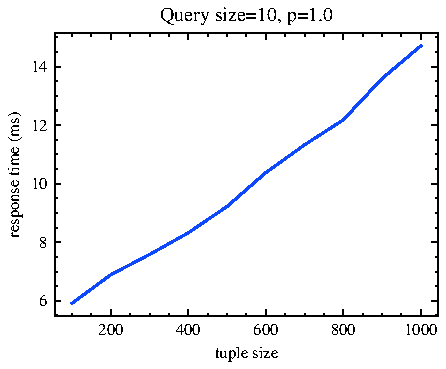
\includegraphics[width=0.6\textwidth]{my/graphics/tuple_completion_3.pdf}
	\caption{Optimal matching response time (ms) w.r.t. varying tuple sizes}
	\label{fig:tuple_completion_3}
\end{figure}

Our workloads A and B have query sizes of 3 and 5, respectively. The average number of attributes of the 10 datasets is less than 200. 
The experiment results from the above three steps indicate that the response time of optimal matching will be less than 30 milliseconds in our use case. 
The performance cost of optimal matching will not be as significant as that of full-text index lookup. 
Therefore, the majority of our work focuses on how to optimize index lookup using neural networks.

\subsection{Neural network based predictive access}
\label{subsection:nn_experiments}

We evaluate five neural network architectures including MLP, LSTM, Conv1D, Transformer and MLP-Mixer. While all of them can be made into deep networks, or in conjunction with other network architectures, our motivation is to make our models as small as possible so that they can be embedded in a search system.
Therefore, we focus on the minimalist approach to network design.

\subsubsection{Common experimental setup and evaluation metrics}
\noindent{\emph {Evaluation scenarios:}}
 We evaluate models with the following combination of different scenarios in all experiments:
\begin{itemize}
	\item We train the models using different sampling rates of attributes, as described in Section~\ref{subsection:training_data_gen}.
	\item We consider both word-based and 3-gram based training.
	\item We evaluate the performance of index scan using models' predictions
	and compare with the optimal and aggregate index lookup for each query in our query workloads.
\end{itemize}

\noindent{\emph {Tokenization and embedding of texts:}}
The tokens are either words or 3-grams of the values in the partial tuples.  Let $\mathbf{Voc}$ be the vocabulary.  The vocabulary size is determined by the attribute sampling rate during training. The vocabulary sizes are given in Table~\ref{tab:training_vocab_size}. Each token is embedded into $\mathbb{R}^{64}$ by a simple embedding layer that has
$|\mathbf{Voc}|\times 64$ parameters.

\noindent{\emph {Evaluation metrics:}}
We evaluate our models using the following metrics:
\begin{itemize}
\item Top-$k$ classification accuracy: since we know the true relations that contain the partial tuples in our query workloads, we can evaluate the classification accuracy of our model.  The top-$k$ accuracy is defined as the percentage of the correct label among the top-$k$ labels predicted.
\item Index lookup response time using the predicted access pattern: using the likelihoods produced by our model, we can sort the indexes by their likelihoods and access the most likely index first. The scan continues until the true relation is reached.
\end{itemize}

\subsubsection{Multilayer perceptron (MLP)}
\label{subsection:expt_mlp}

\noindent{\emph Description:}

Multilayer perceptron (MLP) is probably the most widely used neural network architecture.  In this experiment, we will test the effectiveness of MLP by itself with a single hidden layer.

\noindent{\emph {Model architecture:}}

\begin{itemize}
    \item Since each query is a sequence of tokens, each query is embedded into
    $\mathbb{R}^{L\times 64}$ where $L$ is the token sequence length.  We use global
    average pooling to generate a flat vector in $\mathbb{R}^{64}$, which is used as the input to the MLP layer.
    \item MLP has one hidden layer of size 100.
    \item We utilize one drop-out layer to prevent overfitting by the large embedding layer.
\end{itemize}

The overall network architecture can be found in Figure~\ref{fig:mlp_model}.
\begin{figure}[!th]
	\centering
	\includesvg[inkscapelatex=false, width = 250pt]{mlp_model.svg}
	\caption{MLP model}
	\label{fig:mlp_model}
\end{figure}
Since we have six sets of training datasets, we have 6 trained MLP models, as shown in Table \ref{tab:trained_mlp_models}.
\begin{table}[!th]
	\centering
	\begin{tabularx}{0.8\textwidth}{|l|X|}
		\hline
		\textbf{Model name} & \textbf{Training dataset} \\ \hline
		mlp100 & 100\% attrs., word-based \\
		mlp100-3gram\ & 100\% attrs., 3-gram based \\ 
		mlp75 & 75\% attrs., word-based \\
		mlp75-3gram & 75\% attrs., 3-gram based \\ 
		mlp50 & 50\% attrs., word-based \\
		mlp50-3gram & 50\% attrs., 3-gram based \\ 
		\hline
	\end{tabularx}
	\caption{MLP model names and corresponding training datasets.}
	\label{tab:trained_mlp_models}
\end{table}

\noindent{\emph Observations:}

\begin{itemize}
	\item The top-1 to top-5 accuracies for all variations of MLP models under the workloads A and B are shown in Figure~\ref{fig:top_k_mlp_all}. Word-based models perform better than 3-gram based models under both workloads, which do not contain misspelled and unknown keywords.
	\item Figure~\ref{fig:mlp_perf_all_A} and Figure~\ref{fig:mlp_perf_all_B} show the distribution of query processing time under the workloads A and B, respectively. Word-based models improve query processing more than 3-gram based models do. In addition, the models trained using partial tuples with less attributes perform better than those trained using partial tuples with more attributes.
\end{itemize}
\begin{figure}[!th]
	\centering
	\begin{subfigure}{0.45\textwidth}
		\centering
%		\includesvg[inkscapelatex=false]{top_k_mlp_A.svg}
		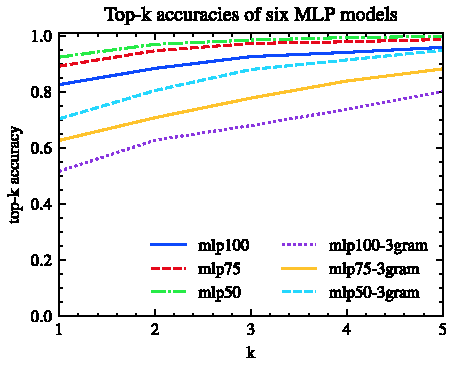
\includegraphics[]{my/graphics/top_k_mlp_A.pdf}
		\caption{Under the workload A.}
		\label{fig:top_k_mlp_A}
	\end{subfigure}
	\hfill
	\begin{subfigure}{0.45\textwidth}
		\centering
%		\includesvg[inkscapelatex=false]{top_k_mlp_B.svg}
		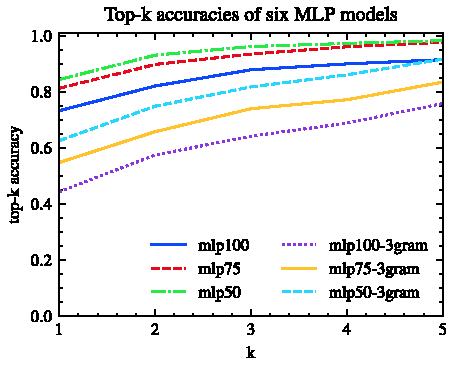
\includegraphics[]{my/graphics/top_k_mlp_B.pdf}
		\caption{Under the workload B.}
		\label{fig:top_k_mlp_B}
	\end{subfigure}
	\caption{Top-$k$ accuracies of six MLP models under the workload A and B.}
	\label{fig:top_k_mlp_all}
\end{figure}
\begin{figure}[!th]
	\centering
	\begin{subfigure}{0.45\textwidth}
		\begin{subfigure}{\textwidth}
			\centering
%			\includesvg[inkscapelatex=false]{perf_dist_mlp100_A.svg}
			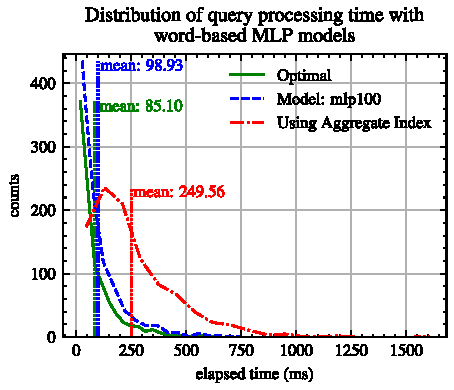
\includegraphics[]{my/graphics/perf_dist_mlp100_A.pdf}
		\end{subfigure}
		\vfill
		\begin{subfigure}{\textwidth}
			\centering
%			\includesvg[inkscapelatex=false]{perf_dist_mlp75_A.svg}
			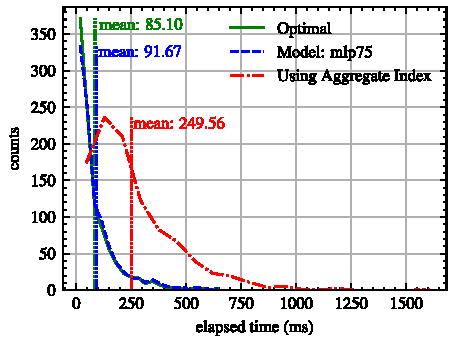
\includegraphics[]{my/graphics/perf_dist_mlp75_A.pdf}
		\end{subfigure}
		\vfill
		\begin{subfigure}{\textwidth}
			\centering
%			\includesvg[inkscapelatex=false]{perf_dist_mlp50_A.svg}
			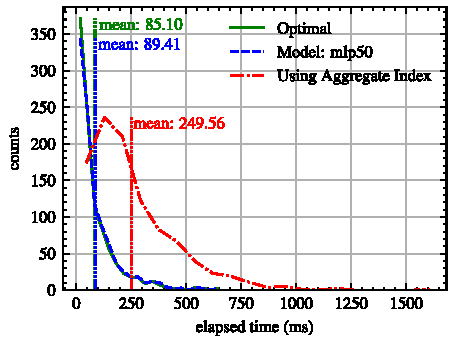
\includegraphics[]{my/graphics/perf_dist_mlp50_A.pdf}
		\end{subfigure}
		\caption{Word-based MLP models}
	\end{subfigure}
	\hfill
	\begin{subfigure}{0.45\textwidth}
		\begin{subfigure}{\textwidth}
			\centering
%			\includesvg[inkscapelatex=false]{perf_dist_mlp100_3gram_A.svg}
			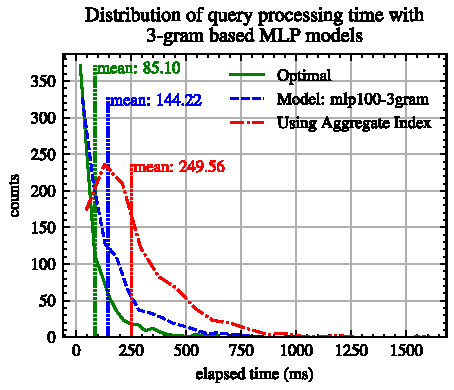
\includegraphics[]{my/graphics/perf_dist_mlp100_3gram_A.pdf}
		\end{subfigure}
		\vfill
		\begin{subfigure}{\textwidth}
			\centering
%			\includesvg[inkscapelatex=false]{perf_dist_mlp75_3gram_A.svg}
			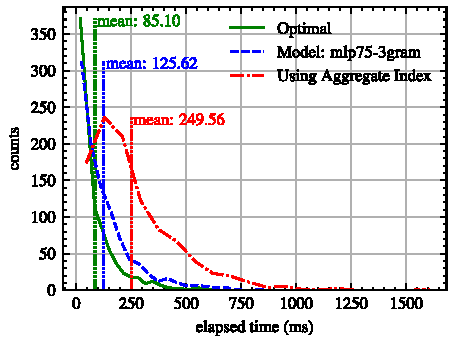
\includegraphics[]{my/graphics/perf_dist_mlp75_3gram_A.pdf}
		\end{subfigure}
		\vfill
		\begin{subfigure}{\textwidth}
			\centering
%			\includesvg[inkscapelatex=false]{perf_dist_mlp50_3gram_A.svg}
			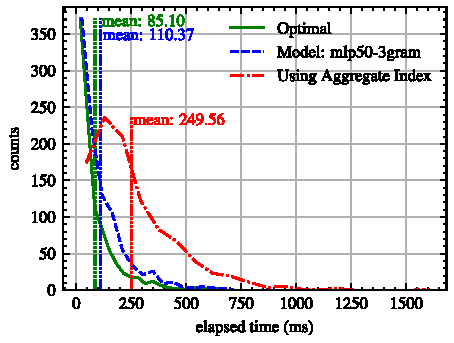
\includegraphics[]{my/graphics/perf_dist_mlp50_3gram_A.pdf}
		\end{subfigure}
		\caption{3-gram based MLP models}
	\end{subfigure}
	\caption{Distribution of query processing time with MLP models under the workload A.}
	\label{fig:mlp_perf_all_A}
\end{figure}
\begin{figure}[!th]
	\centering
	\begin{subfigure}{0.45\textwidth}
		\begin{subfigure}{\textwidth}
			\centering
%			\includesvg[inkscapelatex=false]{perf_dist_mlp100_B.svg}
			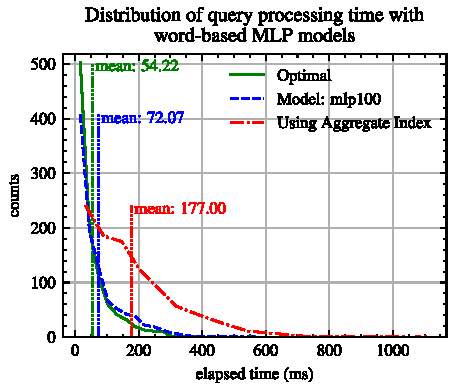
\includegraphics[]{my/graphics/perf_dist_mlp100_B.pdf}
		\end{subfigure}
		\vfill
		\begin{subfigure}{\textwidth}
			\centering
			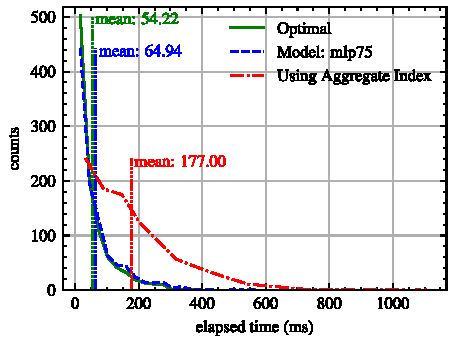
\includegraphics[]{my/graphics/perf_dist_mlp75_B.pdf}
		\end{subfigure}
		\vfill
		\begin{subfigure}{\textwidth}
			\centering
			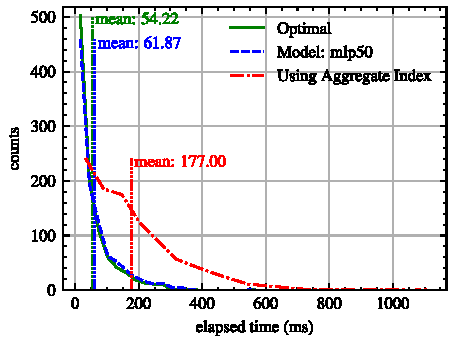
\includegraphics[]{my/graphics/perf_dist_mlp50_B.pdf}
		\end{subfigure}
		\caption{Word-based MLP models}
	\end{subfigure}
	\hfill
	\begin{subfigure}{0.45\textwidth}
		\begin{subfigure}{\textwidth}
			\centering
			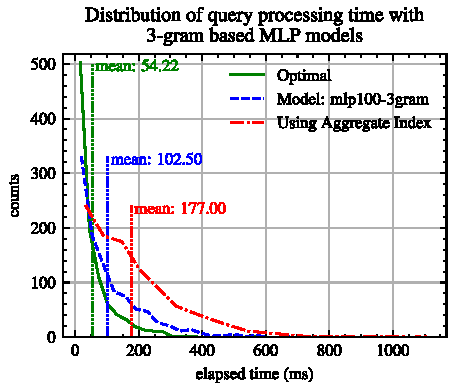
\includegraphics[]{my/graphics/perf_dist_mlp100_3gram_B.pdf}
		\end{subfigure}
		\vfill
		\begin{subfigure}{\textwidth}
			\centering
			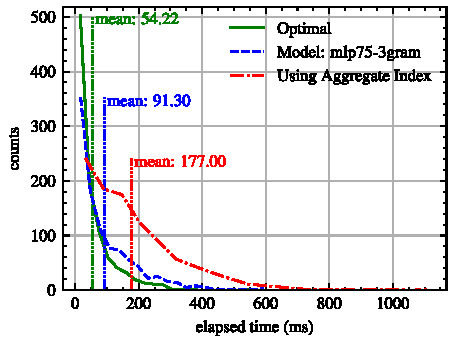
\includegraphics[]{my/graphics/perf_dist_mlp75_3gram_B.pdf}
		\end{subfigure}
		\vfill
		\begin{subfigure}{\textwidth}
			\centering
			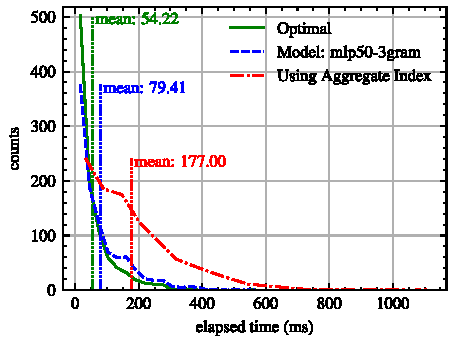
\includegraphics[]{my/graphics/perf_dist_mlp50_3gram_B.pdf}
		\end{subfigure}
		\caption{3-gram based MLP models}
	\end{subfigure}
	\caption{Distribution of query processing time with MLP models under the workload B.}
	\label{fig:mlp_perf_all_B}
\end{figure}

\subsubsection{Long short-term memory (LSTM)}

\noindent{\emph Description:}

Long short-term memory (LSTM) is a neural network architecture for sequence learning. Even though attributes in a tuple is not considered as a sequence since they are not ordered, the attribute values can be considered as short sequences of tokens. We test how LSTM performs when dealing with relational data in this experiment. Again we apply the minimalist approach to its network design by a single LSTM layer.

\noindent{\emph {Model architecture:}}

\begin{itemize}
	\item Each query is embedded into $\mathbb{R}^{L\times 64}$ where $L$ is the token sequence length, which is used as the input to the LSTM layer.
	\item We apply one drop-out layer to the output of the LSTM layer to prevent overfitting.
	\item The LSTM model has one hidden layer of size 100.
\end{itemize}

The model architecture is shown in Figure \ref{fig:lstm_model}. The 6 trained LSTM models are listed in Table~\ref{tab:trained_lstm_models}.
\begin{figure}[!th]
	\centering
	\includesvg[inkscapelatex=false, width = 250pt]{lstm_model.svg}
	\caption{LSTM model}
	\label{fig:lstm_model}
\end{figure}
\begin{table}[!th]
	\centering
	\begin{tabularx}{0.8\textwidth}{|l|X|}
		\hline
		\textbf{Model name} & \textbf{Training dataset} \\ \hline
		lstm100 & 100\% attrs., word-based \\
		lstm100-3gram & 100\% attrs., 3-gram based \\ 
		lstm75 & 75\% attrs., word-based \\
		lstm75-3gram & 75\% attrs., 3-gram based \\ 
		lstm50 & 50\% attrs., word-based \\
		lstm50-3gram & 50\% attrs., 3-gram based \\ 
		\hline
	\end{tabularx}
	\caption{LSTM model names and corresponding training datasets.}
	\label{tab:trained_lstm_models}
\end{table}

\noindent{\emph Observations:}

\begin{itemize}
	\item The top-1 to top-5 accuracies for all variations of LSTM models under the workloads A and B are shown in Figure~\ref{fig:top_k_lstm_all}. 
	Word-based models perform better than 3-gram based models. When compared to MLP models, LSTM models underperform under both workloads.
	\item Figure~\ref{fig:lstm_perf_all_A} and Figure~\ref{fig:lstm_perf_all_B} show the distribution of query processing time under the workloads A and B, respectively. 
	Word-based models improve query processing more than 3-gram based models do. 
	In addition, similar to MLP models, the models trained using partial tuples with less attributes perform better than those trained using partial tuples with more attributes.
\end{itemize}
\begin{figure}[!th]
	\centering
	\begin{subfigure}{0.45\textwidth}
		\centering
%		\includesvg[inkscapelatex=false]{top_k_lstm_A.svg}
		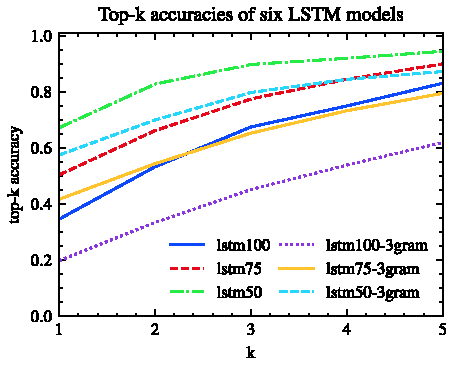
\includegraphics[]{my/graphics/top_k_lstm_A.pdf}
		\caption{Under the workload A.}
		\label{fig:top_k_lstm_A}
	\end{subfigure}
	\hfill
	\begin{subfigure}{0.45\textwidth}
		\centering
		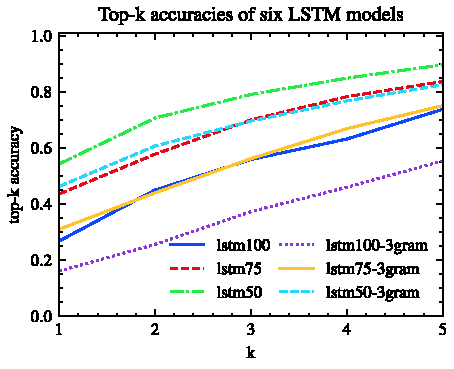
\includegraphics[]{my/graphics/top_k_lstm_B.pdf}
		\caption{Under the workload B.}
		\label{fig:top_k_lstm_B}
	\end{subfigure}
	\caption{Top-$k$ accuracies of six LSTM models under the workload A and B.}
	\label{fig:top_k_lstm_all}
\end{figure}
\begin{figure}[!th]
	\centering
	\begin{subfigure}{0.45\textwidth}
		\begin{subfigure}{\textwidth}
			\centering
%			\includesvg[inkscapelatex=false]{perf_dist_lstm100_A.svg}
			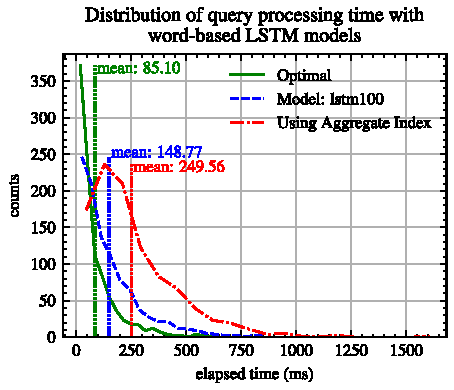
\includegraphics[]{my/graphics/perf_dist_lstm100_A.pdf}
		\end{subfigure}
		\vfill
		\begin{subfigure}{\textwidth}
			\centering
			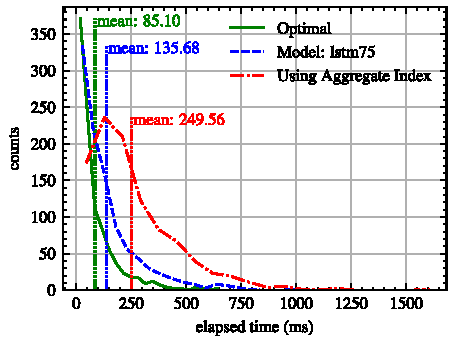
\includegraphics[]{my/graphics/perf_dist_lstm75_A.pdf}
		\end{subfigure}
		\vfill
		\begin{subfigure}{\textwidth}
			\centering
			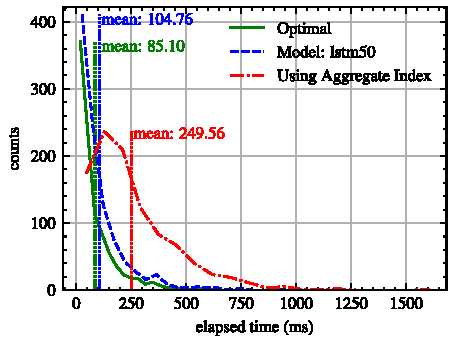
\includegraphics[]{my/graphics/perf_dist_lstm50_A.pdf}
		\end{subfigure}
		\caption{Word-based LSTM models}
	\end{subfigure}
	\hfill
	\begin{subfigure}{0.45\textwidth}
		\begin{subfigure}{\textwidth}
			\centering
			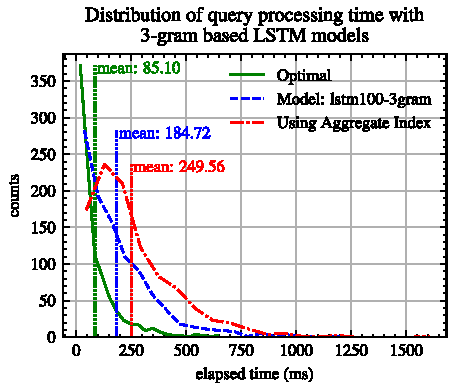
\includegraphics[]{my/graphics/perf_dist_lstm100_3gram_A.pdf}
		\end{subfigure}
		\vfill
		\begin{subfigure}{\textwidth}
			\centering
			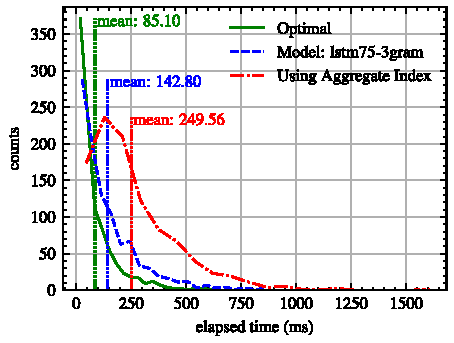
\includegraphics[]{my/graphics/perf_dist_lstm75_3gram_A.pdf}
		\end{subfigure}
		\vfill
		\begin{subfigure}{\textwidth}
			\centering
			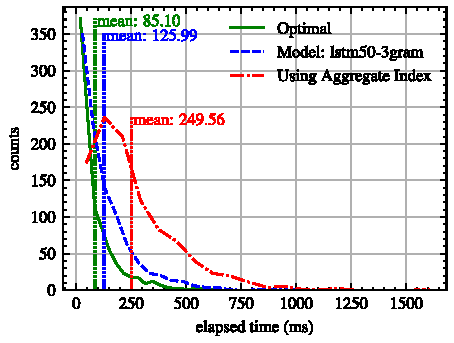
\includegraphics[]{my/graphics/perf_dist_lstm50_3gram_A.pdf}
		\end{subfigure}
		\caption{3-gram based LSTM models}
	\end{subfigure}
	\caption{Distribution of query processing time with LSTM models under the workload A.}
	\label{fig:lstm_perf_all_A}
\end{figure}
\begin{figure}[!th]
	\centering
	\begin{subfigure}{0.45\textwidth}
		\begin{subfigure}{\textwidth}
			\centering
%			\includesvg[inkscapelatex=false]{perf_dist_lstm100_B.svg}
			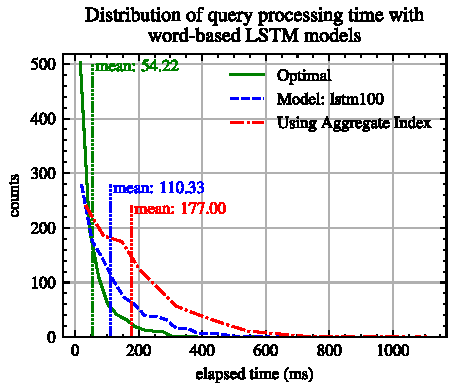
\includegraphics[]{my/graphics/perf_dist_lstm100_B.pdf}
		\end{subfigure}
		\vfill
		\begin{subfigure}{\textwidth}
			\centering
			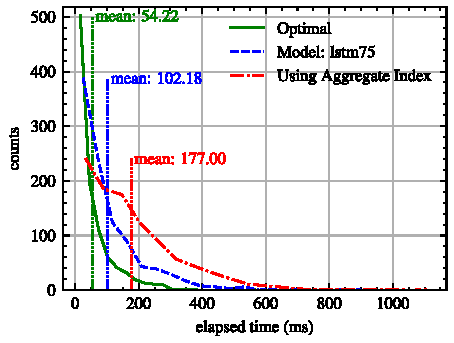
\includegraphics[]{my/graphics/perf_dist_lstm75_B.pdf}
		\end{subfigure}
		\vfill
		\begin{subfigure}{\textwidth}
			\centering
			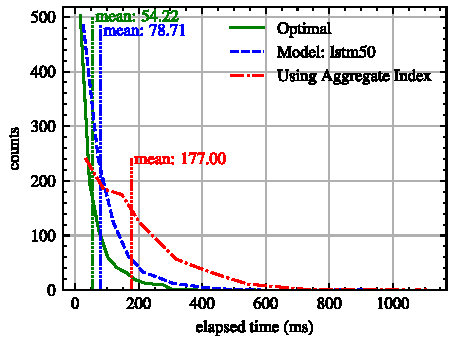
\includegraphics[]{my/graphics/perf_dist_lstm50_B.pdf}
		\end{subfigure}
		\caption{Word-based LSTM models}
	\end{subfigure}
	\hfill
	\begin{subfigure}{0.45\textwidth}
		\begin{subfigure}{\textwidth}
			\centering
			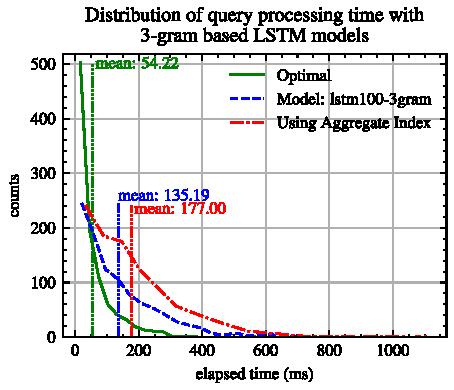
\includegraphics[]{my/graphics/perf_dist_lstm100_3gram_B.pdf}
		\end{subfigure}
		\vfill
		\begin{subfigure}{\textwidth}
			\centering
			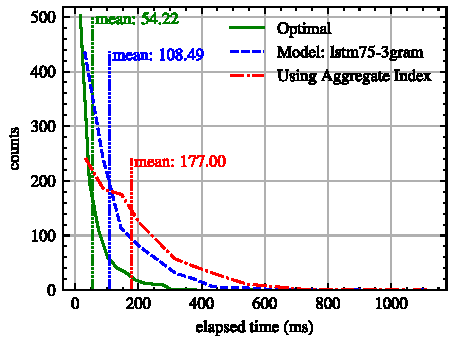
\includegraphics[]{my/graphics/perf_dist_lstm75_3gram_B.pdf}
		\end{subfigure}
		\vfill
		\begin{subfigure}{\textwidth}
			\centering
			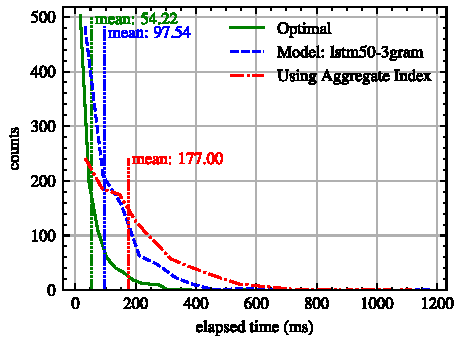
\includegraphics[]{my/graphics/perf_dist_lstm50_3gram_B.pdf}
		\end{subfigure}
		\caption{3-gram based LSTM models}
	\end{subfigure}
	\caption{Distribution of query processing time with LSTM models under the workload B.}
	\label{fig:lstm_perf_all_B}
\end{figure}

\subsubsection{One dimensional convolution (Conv1D)}

\noindent{\emph Description:}

Another way of doing sequence learning is 1-dimensional convolutional neural networks (Conv1D). Similar to what we do to LSTM, we want to see how Conv1D performs when processing relational data. We also minimize the network structure by using a single Conv1D layer.

\noindent{\emph {Model architecture:}}

\begin{itemize}
	\item Each query is embedded into $\mathbb{R}^{L\times 64}$ where $L$ is the token sequence length, which is used as the input to the Conv1D layer.
	\item The Conv1D layer has 64 kernels with kernel size of 3.
	\item We apply global average pooling to the output of Conv1D layer to generate a flat vector in $\mathbb{R}^{64}$.
	\item We apply one drop-out layer to the flattened vector to prevent overfitting.
\end{itemize}

The model architecture is shown in Figure~\ref{fig:conv1d_model}. The 6 trained Conv1D models are listed in Table~\ref{tab:trained_conv1d_models}.
\begin{figure}[!th]
	\centering
	\includesvg[inkscapelatex=false, width = 250pt]{conv1d_model.svg}
	\caption{Conv1D model}
	\label{fig:conv1d_model}
\end{figure}
\begin{table}[!th]
	\centering
	\begin{tabularx}{0.8\textwidth}{|l|X|}
		\hline
		\textbf{Model name} & \textbf{Training dataset} \\ \hline
		conv1d100 & 100\% attrs., word-based \\
		conv1d100-3gram & 100\% attrs., 3-gram based \\ 
		conv1d75 & 75\% attrs., word-based \\
		conv1d75-3gram & 75\% attrs., 3-gram based \\ 
		conv1d50 & 50\% attrs., word-based \\
		conv1d50-3gram & 50\% attrs., 3-gram based \\ 
		\hline
	\end{tabularx}
	\caption{Conv1D model names and corresponding training datasets.}
	\label{tab:trained_conv1d_models}
\end{table}

\noindent{\emph Observations:}

\begin{itemize}
	\item The top-1 to top-5 accuracies for all variations of Conv1D models under the workloads A and B are shown in Figure~\ref{fig:top_k_conv1d_all}. 
	Word-based models perform better than 3-gram based models.
	\item Figure~\ref{fig:conv1d_perf_all_A} and Figure~\ref{fig:conv1d_perf_all_B} show the distribution of query processing time under the workloads A and B, respectively. 
	Word-based models improve query processing more than 3-gram based models do. 
	Under the workload A, the 3-gram based models trained using partial tuples with less attributes perform better than those trained using partial tuples with more attributes, but the word-based models show an opposite relationship.
	Under the workload B, both word-based and 3-gram based models do better when trained using partial tuples with less attributes.
\end{itemize}
\begin{figure}[!th]
	\centering
	\begin{subfigure}{0.45\textwidth}
		\centering
		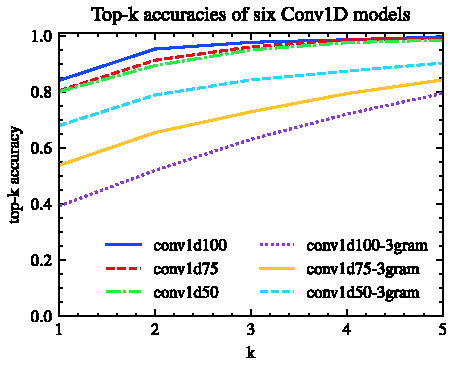
\includegraphics[]{my/graphics/top_k_conv1d_A.pdf}
		\caption{Under the workload A.}
		\label{fig:top_k_conv1d_A}
	\end{subfigure}
	\hfill
	\begin{subfigure}{0.45\textwidth}
		\centering
		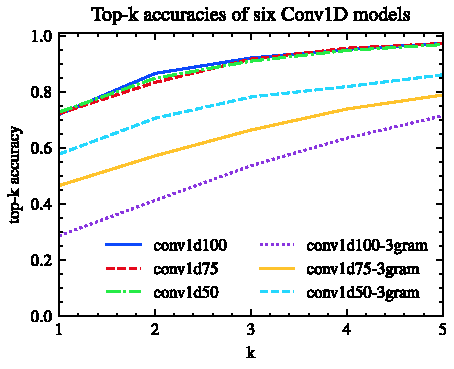
\includegraphics[]{my/graphics/top_k_conv1d_B.pdf}
		\caption{Under the workload B.}
		\label{fig:top_k_conv1d_B}
	\end{subfigure}
	\caption{Top-$k$ accuracies of six Conv1D models under the workload A and B.}
	\label{fig:top_k_conv1d_all}
\end{figure}
\begin{figure}[!h]
	\centering
	\begin{subfigure}{0.45\textwidth}
		\begin{subfigure}{\textwidth}
			\centering
			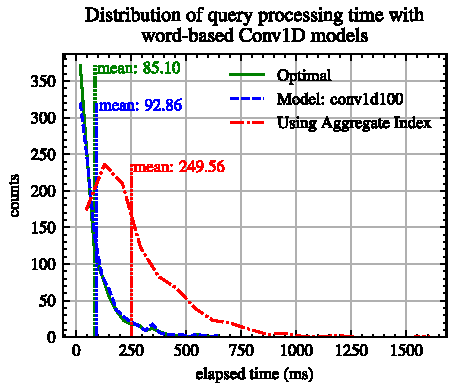
\includegraphics[]{my/graphics/perf_dist_conv1d100_A.pdf}
		\end{subfigure}
		\vfill
		\begin{subfigure}{\textwidth}
			\centering
			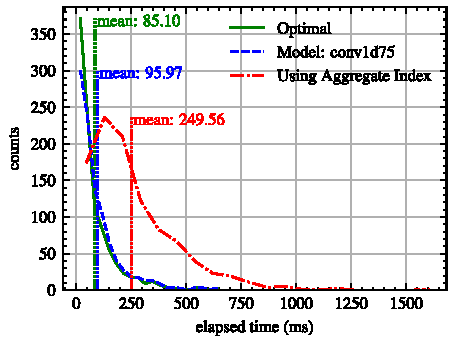
\includegraphics[]{my/graphics/perf_dist_conv1d75_A.pdf}
		\end{subfigure}
		\vfill
		\begin{subfigure}{\textwidth}
			\centering
			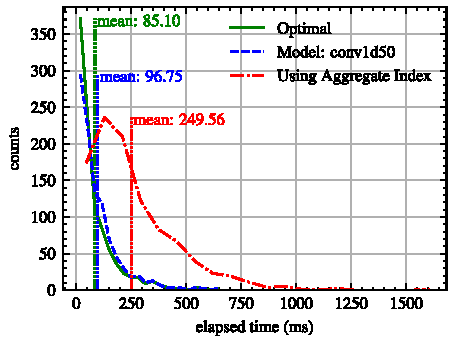
\includegraphics[]{my/graphics/perf_dist_conv1d50_A.pdf}
		\end{subfigure}
		\caption{Word-based Conv1D models}
	\end{subfigure}
	\hfill
	\begin{subfigure}{0.45\textwidth}
		\begin{subfigure}{\textwidth}
			\centering
			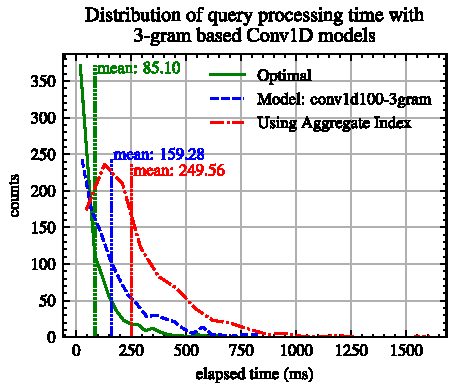
\includegraphics[]{my/graphics/perf_dist_conv1d100_3gram_A.pdf}
		\end{subfigure}
		\vfill
		\begin{subfigure}{\textwidth}
			\centering
			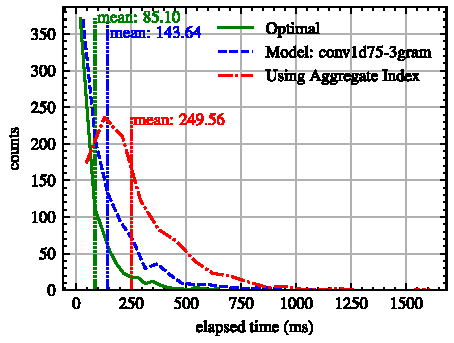
\includegraphics[]{my/graphics/perf_dist_conv1d75_3gram_A.pdf}
		\end{subfigure}
		\vfill
		\begin{subfigure}{\textwidth}
			\centering
			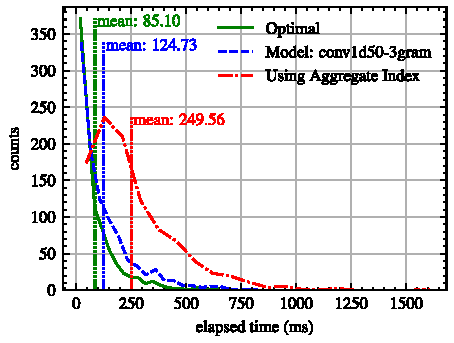
\includegraphics[]{my/graphics/perf_dist_conv1d50_3gram_A.pdf}
		\end{subfigure}
		\caption{3-gram based Conv1D models}
	\end{subfigure}
	\caption{Distribution of query processing time with Conv1D models under the workload A.}
	\label{fig:conv1d_perf_all_A}
\end{figure}
\begin{figure}[!h]
	\centering
	\begin{subfigure}{0.45\textwidth}
		\begin{subfigure}{\textwidth}
			\centering
			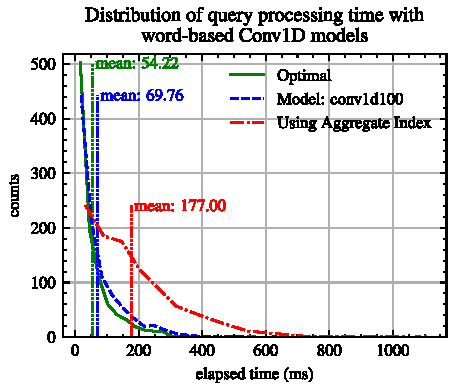
\includegraphics[]{my/graphics/perf_dist_conv1d100_B.pdf}
		\end{subfigure}
		\vfill
		\begin{subfigure}{\textwidth}
			\centering
			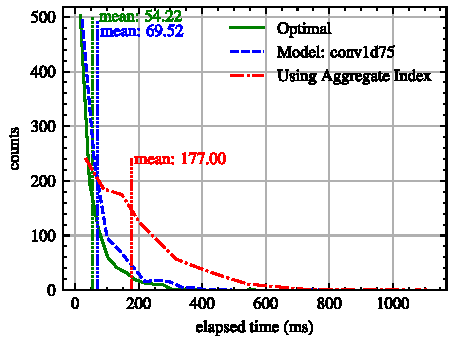
\includegraphics[]{my/graphics/perf_dist_conv1d75_B.pdf}
		\end{subfigure}
		\vfill
		\begin{subfigure}{\textwidth}
			\centering
			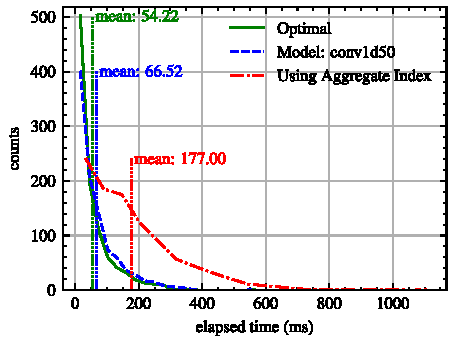
\includegraphics[]{my/graphics/perf_dist_conv1d50_B.pdf}
		\end{subfigure}
		\caption{Word-based Conv1D models}
	\end{subfigure}
	\hfill
	\begin{subfigure}{0.45\textwidth}
		\begin{subfigure}{\textwidth}
			\centering
			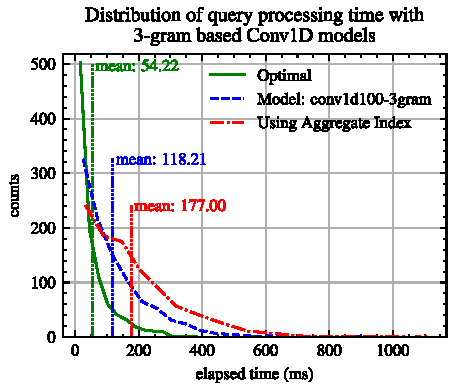
\includegraphics[]{my/graphics/perf_dist_conv1d100_3gram_B.pdf}
		\end{subfigure}
		\vfill
		\begin{subfigure}{\textwidth}
			\centering
			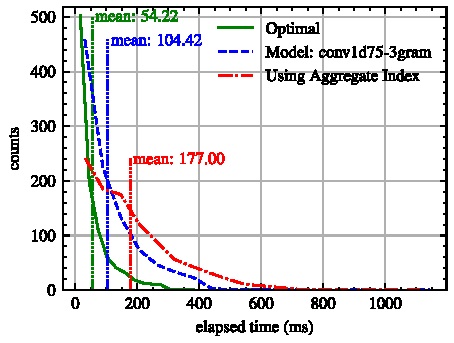
\includegraphics[]{my/graphics/perf_dist_conv1d75_3gram_B.pdf}
		\end{subfigure}
		\vfill
		\begin{subfigure}{\textwidth}
			\centering
			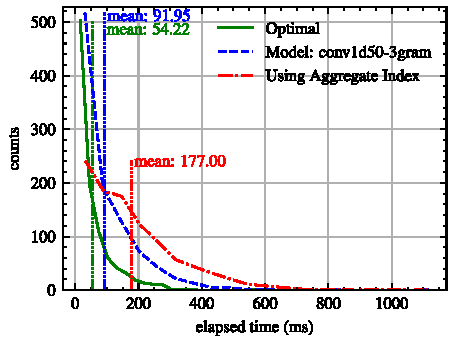
\includegraphics[]{my/graphics/perf_dist_conv1d50_3gram_B.pdf}
		\end{subfigure}
		\caption{3-gram based Conv1D models}
	\end{subfigure}
	\caption{Distribution of query processing time with Conv1D models under the workload B.}
	\label{fig:conv1d_perf_all_B}
\end{figure}

\subsubsection{Single transformer block}

\noindent{\emph Description:}

The Transformer architecture introduced in the original Transformer paper \cite{DBLP:journals/corr/VaswaniSPUJGKP17} is one of the main advances in natural language processing. In this experiment, we evaluate Transformer architecture for relational data. We largely follow the encoder architecture of the vanilla Transformer presented in the paper \cite{DBLP:journals/corr/VaswaniSPUJGKP17}. However, since our data are relational, we remove positional encoding. In addition, we only create one Transformer block to minimize the model architecture.

\noindent{\emph {Model architecture:}}

\begin{itemize}
	\item Each query is embedded into $\mathbb{R}^{L\times 64}$ where $L$ is the token sequence length, which is used as the input to the Transformer block.
	\item Inside the Transformer block, the attention layer has 4 attention heads. We add an extra drop-out layer after both the attention layer and the feed-forward network to prevent overfitting.
	\item The feed-forward network has a hidden layer of size 64.
	\item We apply global average pooling to the output of the Transformer block to generate a flat vector in $\mathbb{R}^{64}$.
        \item Then we apply a drop-out layer to the flattened vector.
\end{itemize}

Figure \ref{fig:transformer_model_all} shows its architecture. The 6 trained Transformer models are listed in Table~\ref{tab:trained_transformer_models}.
\begin{figure}[!th]
	\begin{subfigure}[]{0.4\textwidth}
		\begin{subfigure}[]{\textwidth}
			\centering
			\includesvg[inkscapelatex=false, width = \textwidth]{transformer_model.svg}
			\caption{Overall architecture}
			\label{fig:transformer_model}		
		\end{subfigure}
		\vfill
		\begin{subfigure}[]{\textwidth}
			\centering
			\includesvg[inkscapelatex=false, width = \textwidth]{transformer_model_ffn.svg}
			\caption{Feed-forward network}
			\label{fig:transformer_model_ffn}
		\end{subfigure}
	\end{subfigure}
	\hfill
	\centering
	\begin{subfigure}[]{0.5\textwidth}
		\centering
		\includesvg[inkscapelatex=false, width = \textwidth]{transformer_model_block.svg}
		\caption{Transformer block}
		\label{fig:transformer_model_block}
	\end{subfigure}
	\caption{Transformer model}
	\label{fig:transformer_model_all}
\end{figure}

\begin{table}[!th]
	\centering
	\begin{tabularx}{0.8\textwidth}{|l|X|}
		\hline
		\textbf{Model name} & \textbf{Training dataset} \\ \hline
		transformer100 & 100\% attrs., word-based \\
		transformer100-3gram & 100\% attrs., 3-gram based \\ 
		transformer75 & 75\% attrs., word-based \\
		transformer75-3gram & 75\% attrs., 3-gram based \\ 
		transformer50 & 50\% attrs., word-based \\
		transformer50-3gram & 50\% attrs., 3-gram based \\ 
		\hline
	\end{tabularx}
	\caption{Transformer model names and corresponding training datasets.}
	\label{tab:trained_transformer_models}
\end{table}
\noindent{\emph Observations:}

\begin{itemize}
	\item The top-1 to top-5 accuracies for all variations of Transformer models under the workloads A and B are shown in Figure~\ref{fig:top_k_transformer_all}. 
	Again, word-based models perform better than 3-gram based models. 
	\item Figure~\ref{fig:transformer_perf_all_A} and Figure~\ref{fig:transformer_perf_all_B} show the distribution of query processing time under the workloads A and B, respectively.
	Word-based models improve query processing more than 3-gram based models do.
	In addition, the models trained using partial tuples with less attributes perform better than those trained using partial tuples with more attributes.
\end{itemize}
\begin{figure}[!th]
	\centering
	\begin{subfigure}{0.45\textwidth}
		\centering
		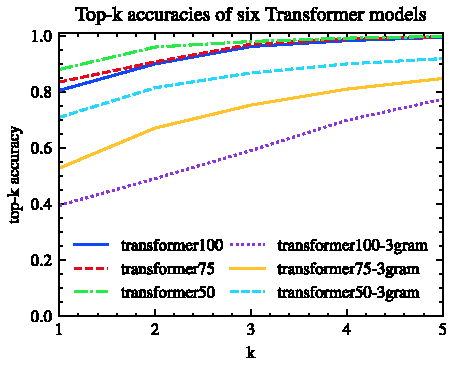
\includegraphics[]{my/graphics/top_k_transformer_A.pdf}
		\caption{Under the workload A.}
		\label{fig:top_k_transformer_A}
	\end{subfigure}
	\hfill
	\begin{subfigure}{0.45\textwidth}
		\centering
		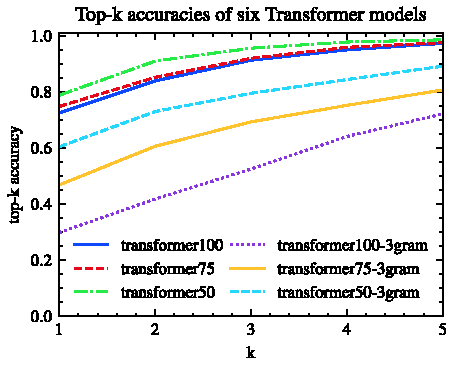
\includegraphics[]{my/graphics/top_k_transformer_B.pdf}
		\caption{Under the workload B.}
		\label{fig:top_k_transformer_B}
	\end{subfigure}
	\caption{Top-$k$ accuracies of six Transformer models under the workload A and B.}
	\label{fig:top_k_transformer_all}
\end{figure}
\begin{figure}[p]
	\centering
	\begin{subfigure}{0.45\textwidth}
		\begin{subfigure}{\textwidth}
			\centering
			\includegraphics[]{my/graphics/perf_dist_transformer100_A.pdf}
		\end{subfigure}
		\vfill
		\begin{subfigure}{\textwidth}
			\centering
			\includegraphics[]{my/graphics/perf_dist_transformer75_A.pdf}
		\end{subfigure}
		\vfill
		\begin{subfigure}{\textwidth}
			\centering
			\includegraphics[]{my/graphics/perf_dist_transformer50_A.pdf}
		\end{subfigure}
		\caption{Word-based Transformer models}
	\end{subfigure}
	\hfill
	\begin{subfigure}{0.45\textwidth}
		\begin{subfigure}{\textwidth}
			\centering
			\includegraphics[]{my/graphics/perf_dist_transformer100_3gram_A.pdf}
		\end{subfigure}
		\vfill
		\begin{subfigure}{\textwidth}
			\centering
			\includegraphics[]{my/graphics/perf_dist_transformer75_3gram_A.pdf}
		\end{subfigure}
		\vfill
		\begin{subfigure}{\textwidth}
			\centering
			\includegraphics[]{my/graphics/perf_dist_transformer50_3gram_A.pdf}
		\end{subfigure}
		\caption{3-gram based Transformer models}
	\end{subfigure}
	\caption{Distribution of query processing time with Transformer models under the workload A.}
	\label{fig:transformer_perf_all_A}
\end{figure}
\begin{figure}[p]
	\centering
	\begin{subfigure}{0.45\textwidth}
		\begin{subfigure}{\textwidth}
			\centering
			\includegraphics[]{my/graphics/perf_dist_transformer100_B.pdf}
		\end{subfigure}
		\vfill
		\begin{subfigure}{\textwidth}
			\centering
			\includegraphics[]{my/graphics/perf_dist_transformer75_B.pdf}
		\end{subfigure}
		\vfill
		\begin{subfigure}{\textwidth}
			\centering
			\includegraphics[]{my/graphics/perf_dist_transformer50_B.pdf}
		\end{subfigure}
		\caption{Word-based Transformer models}
	\end{subfigure}
	\hfill
	\begin{subfigure}{0.45\textwidth}
		\begin{subfigure}{\textwidth}
			\centering
			\includegraphics[]{my/graphics/perf_dist_transformer100_3gram_B.pdf}
		\end{subfigure}
		\vfill
		\begin{subfigure}{\textwidth}
			\centering
			\includegraphics[]{my/graphics/perf_dist_transformer75_3gram_B.pdf}
		\end{subfigure}
		\vfill
		\begin{subfigure}{\textwidth}
			\centering
			\includegraphics[]{my/graphics/perf_dist_transformer50_3gram_B.pdf}
		\end{subfigure}
		\caption{3-gram based Transformer models}
	\end{subfigure}
	\caption{Distribution of query processing time with Transformer models under the workload B.}
	\label{fig:transformer_perf_all_B}
\end{figure}

\subsubsection{MLP-Mixer}
\label{subsection:expt_mlpmixer}

\noindent{\emph Description:}

MLP-Mixer is an architecture based on MLPs only, which is proposed by Tolstikhin et al. \cite{DBLP:journals/corr/abs-2105-01601}. It is intended for computer vision. However, we want to see whether we could use it for our use case. In this experiment, we modify its architecture for text processing. The same minimalist approach and evaluation scenarios are used as in other experiments.

\noindent{\emph {Model architecture:}}

\begin{itemize}
	\item Each query is embedded into $\mathbb{R}^{L\times 64}$ where $L$ is the token sequence length, which is used as the input to the Mixer Layer.
	\item The Mixer Layer is implemented following the architecture presented in the paper \cite{DBLP:journals/corr/abs-2105-01601}.
	\item Layer normalization is applied to outputs from the Mixer Layer.
	\item We apply global max pooling to the outputs of layer normalization to generate a flat vector in $\mathbb{R}^{64}$, which is used as input to the output layer.
\end{itemize}
Figure \ref{fig:mlpmixer_model_all} shows its architecture. The 6 trained MLP-Mixer models are listed in Table~\ref{tab:trained_mlpmixer_models}.
\begin{figure}[p]
	\centering
	\begin{subfigure}{\textwidth}
		\begin{subfigure}[t]{0.45\textwidth}
			\centering
			\includesvg[inkscapelatex=false, width=\textwidth]{mlpmixer_model_token_mixing.svg}
			\caption{Token mixing}
			\label{fig:mlpmixer_model_token_mixing}
		\end{subfigure}
		\hfill
		\begin{subfigure}[t]{0.45\textwidth}
			\centering
			\includesvg[inkscapelatex=false, width=\textwidth]{mlpmixer_model_channel_mixing.svg}
			\caption{Channel mixing}
			\label{fig:mlpmixer_model_channel_mixing}
		\end{subfigure}
	\end{subfigure}
	\vfill
	\begin{subfigure}{\textwidth}
		\begin{subfigure}[b]{0.4\textwidth}
			\centering
			\includesvg[inkscapelatex=false, width=\textwidth]{mlpmixer_model_mixer.svg}
			\caption{Mixer Layer}
			\label{fig:mlpmixer_model_mixer}
		\end{subfigure}
		\hfill
		\begin{subfigure}[b]{0.4\textwidth}
			\centering
			\includesvg[inkscapelatex=false, width=\textwidth]{mlpmixer_model.svg}
			\caption{Overall architecture}
			\label{fig:mlpmixer_model}
		\end{subfigure}
	\end{subfigure}
	\caption{MLP-Mixer model}
	\label{fig:mlpmixer_model_all}
\end{figure}
\begin{table}[!th]
	\centering
	\begin{tabularx}{0.8\textwidth}{|l|X|}
		\hline
		\textbf{Model name} & \textbf{Training dataset} \\ \hline
		mlpmixer100 & 100\% attrs., word-based \\
		mlpmixer100-3gram & 100\% attrs., 3-gram based \\ 
		mlpmixer75 & 75\% attrs., word-based \\
		mlpmixer75-3gram & 75\% attrs., 3-gram based \\ 
		mlpmixer50 & 50\% attrs., word-based \\
		mlpmixer50-3gram & 50\% attrs., 3-gram based \\ 
		\hline
	\end{tabularx}
	\caption{MLP-Mixer model names and corresponding training datasets.}
	\label{tab:trained_mlpmixer_models}
\end{table}

\noindent{\emph Observations:}

\begin{itemize}
	\item The top-1 to top-5 accuracies for all variations of MLP-Mixer models under the workloads A and B are shown in Figure~\ref{fig:top_k_mlpmixer_all}.
	\item Figure~\ref{fig:mlpmixer_perf_all_A} and Figure~\ref{fig:mlpmixer_perf_all_B} show the distribution of query processing time under the workloads A and B, respectively.
	The word-based models perform slightly better than 3-gram based models, with the exception of two models $\emph mlpmixer75$ and $\emph mlpmixer75$-$3gram$.
	In addition, the models trained using partial tuples with less attributes perform better than those trained using partial tuples with more attributes, 
	with the exception of the model $\emph mlpmixer75$ under the workload B.
\end{itemize}
\begin{figure}[!th]
	\centering
	\begin{subfigure}{0.45\textwidth}
		\centering
		\includegraphics[]{my/graphics/top_k_mlpmixer_A.pdf}
		\caption{Under the workload A.}
		\label{fig:top_k_mlpmixer_A}
	\end{subfigure}
	\hfill
	\begin{subfigure}{0.45\textwidth}
		\centering
		\includegraphics[]{my/graphics/top_k_mlpmixer_B.pdf}
		\caption{Under the workload B.}
		\label{fig:top_k_mlpmixer_B}
	\end{subfigure}
	\caption{Top-$k$ accuracies of six MLP-Mixer models under the workload A and B.}
	\label{fig:top_k_mlpmixer_all}
\end{figure}
\begin{figure}[!h]
	\centering
	\begin{subfigure}{0.45\textwidth}
		\begin{subfigure}{\textwidth}
			\centering
			\includegraphics[]{my/graphics/perf_dist_mlpmixer100_A.pdf}
		\end{subfigure}
		\vfill
		\begin{subfigure}{\textwidth}
			\centering
			\includegraphics[]{my/graphics/perf_dist_mlpmixer75_A.pdf}
		\end{subfigure}
		\vfill
		\begin{subfigure}{\textwidth}
			\centering
			\includegraphics[]{my/graphics/perf_dist_mlpmixer50_A.pdf}
		\end{subfigure}
		\caption{Word-based MLP-Mixer models}
	\end{subfigure}
	\hfill
	\begin{subfigure}{0.45\textwidth}
		\begin{subfigure}{\textwidth}
			\centering
			\includegraphics[]{my/graphics/perf_dist_mlpmixer100_3gram_A.pdf}
		\end{subfigure}
		\vfill
		\begin{subfigure}{\textwidth}
			\centering
			\includegraphics[]{my/graphics/perf_dist_mlpmixer75_3gram_A.pdf}
		\end{subfigure}
		\vfill
		\begin{subfigure}{\textwidth}
			\centering
			\includegraphics[]{my/graphics/perf_dist_mlpmixer50_3gram_A.pdf}
		\end{subfigure}
		\caption{3-gram based MLP-Mixer models}
	\end{subfigure}
	\caption{Distribution of query processing time with MLP-Mixer models under the workload A.}
	\label{fig:mlpmixer_perf_all_A}
\end{figure}
\begin{figure}[!h]
	\centering
	\begin{subfigure}{0.45\textwidth}
		\begin{subfigure}{\textwidth}
			\centering
			\includegraphics[]{my/graphics/perf_dist_mlpmixer100_B.pdf}
		\end{subfigure}
		\vfill
		\begin{subfigure}{\textwidth}
			\centering
			\includegraphics[]{my/graphics/perf_dist_mlpmixer75_B.pdf}
		\end{subfigure}
		\vfill
		\begin{subfigure}{\textwidth}
			\centering
			\includegraphics[]{my/graphics/perf_dist_mlpmixer50_B.pdf}
		\end{subfigure}
		\caption{Word-based MLP-Mixer models}
	\end{subfigure}
	\hfill
	\begin{subfigure}{0.45\textwidth}
		\begin{subfigure}{\textwidth}
			\centering
			\includegraphics[]{my/graphics/perf_dist_mlpmixer100_3gram_B.pdf}
		\end{subfigure}
		\vfill
		\begin{subfigure}{\textwidth}
			\centering
			\includegraphics[]{my/graphics/perf_dist_mlpmixer75_3gram_B.pdf}
		\end{subfigure}
		\vfill
		\begin{subfigure}{\textwidth}
			\centering
			\includegraphics[]{my/graphics/perf_dist_mlpmixer50_3gram_B.pdf}
		\end{subfigure}
		\caption{3-gram based MLP-Mixer models}
	\end{subfigure}
	\caption{Distribution of query processing time with MLP-Mixer models under the workload B.}
	\label{fig:mlpmixer_perf_all_B}
\end{figure}

\subsubsection{Comparison of different models}

Based on the observations from Section~\ref{subsection:expt_mlp} to Section~\ref{subsection:expt_mlpmixer}, we have compiled the following table to compare their relative performances with respect to the optimal and the aggregate index lookup under the workload A.

\begin{table}[ht]
    \centering
    \begin{tabularx}{\textwidth}{|l|X||X|X||X|X|X|}
    \hline
    &    \multicolumn{3}{|c|}{Word tokens} & \multicolumn{3}{|c|}{3-gram tokens} \\ \hline
    Model 
        & parameters
        & $\frac{\mathrm{model}}{\mathrm{optimal}}$
        & $\frac{\mathrm{model}}{\mathrm{aggr}}$ 
        & parameters
        & $\frac{\mathrm{model}}{\mathrm{optimal}}$
        & $\frac{\mathrm{model}}{\mathrm{aggr}}$
        \\ \hline
    MLP & 3.02M & {\bf 1.10} & 0.37 & 272K & {\bf 1.49} & 0.51\\
    LSTM & 3.05M & 1.52 & 0.52 & 305K & 1.78 & 0.61 \\
    Conv1D & 3.03M & {\bf 1.12} & 0.38 & 277K & 1.68 & 0.57 \\
    Transformer & 3.09M & {\bf 1.12} & 0.38 & 340K & {\bf 1.66} & 0.57 \\
    MLP Mixer & 3.04M & 1.65 & 0.56 & 287K & {\bf 1.65} & 0.56 \\ \hline
    \end{tabularx}
    \caption{Comparison of models under the workload A with the top-3 measurements highlighted.}
    \label{tab:model-comparison}
\end{table}

The observation supports our proposal of utilizing neural networks to accelerate
index lookup.  As shown in Table~\ref{tab:model-comparison}, many of the models perform well compared to the optimal index lookup, and significantly outperform the aggregate index lookup.

For word based tokens, MLP is only 10\% slower than the optimal index lookup, and outperforms the aggregate index by almost 3 times. The Conv1D and Transformer are only slightly worse than MLP. But the transformer models have larger model sizes. Both LSTM and MLP Mixer do not perform that well when compared to the other three networks.

We realize that we only use one transformer block and one MLP Mixer Layer, respectively.  In our context, we are interested in embedded networks as part of the query processor. Therefore, our focus is limited to small network architectures.

Regarding the model sizes, the main source of parameters is the embedding layer.
Word based tokens produce far more bigger vocabulary, which then requires many more
embedding vectors as model parameters.  The vocabulary of 3-grams is much smaller, and thus produces much more compact models.

Since 3-gram tokens individually capture less information than word-based tokens, we expect the observed performance degradation when using the 3-gram tokens. With that being said, MLP has shown to outperform the aggregate index with twice the performance even for 3-grams.

The value of 3-gram vocabularies becomes more apparent in scenarios with noisy queries.  When query strings contain spelling and other noises at a sub-word level, the two methods of tokenization, i.e., word-based and 3-gram based, behave quite differently.
For word-based tokenization, noisy words will generate out-of-vocabulary (OOV) tokens
which do not contribute to the classification of the network.  However, the 3-gram tokenization can still produce {\em some} 3-gram tokens even for misspelled and unknown words in a query string.  The next section is dedicated to evaluate how well word-based and 3-gram based networks behave in the presence of noisy queries.

\subsection{Impact of noisy queries on models' performance}
\label{subsection:expt_3gram_resiliency}

\noindent{\emph Descriptions:}

In this experiment, we investigate the impact of misspelled words in queries on the models' performance of top-5 accuracy. We simulate the scenario by replacing a randomly selected character in a word with the special character ``\_". For example, the city name \verb|toronto| becomes \verb|to_onto| after mutation. Its 3-gram tokens will be \verb|[__t, _to, to_, o_o, _on, ont, nto, to_, o__]|.

\noindent{\emph {Observations:}}

The impact of noisy queries on models' performance of top-5 accuracy is shown in Figure \ref{fig:acc_degradation_workload_A_all} and \ref{fig:acc_degradation_workload_B_all}  under  the workload A and B, respectively. The performance degradation of word-based models is much faster than that of 3-gram based models. This clearly shows that 3-gram based models are more resilient to query noises.
\begin{figure}[!th]
	\centering
	\begin{subfigure}[t]{0.95\textwidth}
		\includegraphics[]{my/graphics/acc_degradation_word_based_A.pdf}
		\caption{Word-based models}
		\label{fig:acc_degradation_workload_A_word_based}
	\end{subfigure}
	\vfill
	\begin{subfigure}[t]{0.95\textwidth}
		\includegraphics[]{my/graphics/acc_degradation_3gram_based_A.pdf}
		\caption{3-gram based models}
		\label{fig:acc_degradation_workload_A_3gram}
	\end{subfigure}
	\caption{Top-5 accuracy degradation of all models under the workload A.}
	\label{fig:acc_degradation_workload_A_all}
\end{figure}
\begin{figure}[!th]
	\centering
	\begin{subfigure}[]{0.95\textwidth}
		\includegraphics[]{my/graphics/acc_degradation_word_based_B.pdf}
		\caption{Word-based models}
		\label{fig:acc_degradation_workload_B_word_based}
	\end{subfigure}
	\vfill
	\begin{subfigure}[]{0.95\textwidth}
		\includegraphics[]{my/graphics/acc_degradation_3gram_based_B.pdf}
		\caption{3-gram based models}
		\label{fig:acc_degradation_workload_B_3gram}
	\end{subfigure}
	\caption{Top-5 accuracy degradation of all models under the workload B3.}
	\label{fig:acc_degradation_workload_B_all}
\end{figure}

